\section{Lecture 14: Instrumental Variables Continued}{Jaeeun Park \& Zekai Wang \& Claire Hsu \& Jiarong Zhou(revisions)}
\subsection{Review from Last Lecture}
Last lecture we introduced the notion of instrumental variable and gave a high level definition for it. Assume \(Z\) is the binary instrumental variable (e.g., treatment assigned), \(D\) is the binary treatment a unit actually received, \(Y\) is the outcome, and \(U\) are (unmeasured) confounders that affect both the treatment received and the outcome. 
\begin{center}
    \begin{tikzpicture}
      \node (Z) at (0,0) {$Z$};
      \node (D) at (2,0) {$D$};
      \node (Y) at (4,0) {$Y$};
      \node (U) at (3,1) {$U$};
      
      \draw[->] (Z) -- (D);
      \draw[->] (D) -- (Y);
      \draw[->] (U) -- (D);
      \draw[->] (U) -- (Y);
  \end{tikzpicture}
\end{center}

\begin{definition}
    Informally, the Instrumental Variable (IV) \(Z\) is valid if it meets the following three conditions:
    \begin{enumerate}
        \item Relevance: \(Z\) has a direct effect on \(D\). This can be seen from the \(Z \to D\) path in the causal DAG. 
        \item Exclusion Restriction: \(Z\) only affects \(Y\) through \(D\). This can be seen from the lack of a \(Z \to Y\) path in the causal DAG. 
        \item Exchangeability (Unconfoundness): \(Z\) and \(Y\) don't share unmeasured confounders. This can be seen from the lack of a \(U \to Z\) path in the causal DAG. 
    \end{enumerate}
\end{definition}

As a concrete example, in the Minneapolis Domestic Violence Experiment, police officers are randomly assigned to one of three penalties (arrest, counseling, and separation from partner) when dealing with domestic violence perpetrators. However, officers are not required to strictly follow the assignment. In this example, \(Z\) is the random assignment of the three penalties, \(D\) is the actual penalty given, \(Y\) is the indicator for re-offense, and \(U\) is some latent cause (e.g., propensity to commit violence, severity of the offense). \textit{Relevance} holds since the officers are encouraged to follow the penalty assignment, \textit{Exclusion Restriction} holds since it is reasonable to assume the assignment does not directly affect the chances of re-offense, and \textit{Exchangeability} holds by design since \(Z\) is randomly assigned in the experiment. However, as we will see later, it is usually hard to identify a valid IV in observational studies since doing so involves making untestable assumptions.


\subsection{Instrumental Variables}

\subsubsection{Formal Definition of IV}
To rigorously analyze IVs, we first need to introduce some additional notations. 
\begin{itemize}
    \item \(D(Z = z)\) is the potential outcomes for \(D\), i.e., what treatment a unit would actually receive if the IV takes value $z$. In the Minneapolis Domestic Violence Experiment, this is what penalty would be chosen if the officer is suggested to give penalty \(z\). In the case of binary outcome, we often abbreviate \(D(Z = 1) = D(1), D(Z = 0) = D(0)\).
    \item \(Y(D = d)\) is the potential outcomes for \(Y\) given the unit actually receives treatment \(d\). In the Minneapolis Domestic Violence Experiment, this is the indicator for re-offense if the officer gives penalty \(d\) to the perpetrator. 
    \item \(Y(Z = z, D = d)\) is the potential outcomes for \(Y\) given the unit has IV value \(z\) and actually receives treatment \(d\). In the Minneapolis Domestic Violence Experiment, this is the indicator for re-offense if the officer is suggested to give penalty \(z\) and actually gives penalty \(d\). 
    \item \(Y(Z = z) = Y(Z = z, D = D(Z = z))\) is the potential outcomes we would observe if a unit has IV value $z$. In the Minneapolis Domestic Violence Experiment, this is the indicator for re-offense if the officer is suggested to give penalty \(z\) but we don't have information about what penalty the officer actually gives. 
\end{itemize}
With these, we are ready to formally define IVs. 
\begin{definition}
    A variable \(Z\) is a valid Instrumental Variable (IV) if it satisfies the following three conditions:  
    \begin{enumerate}
        \item \textbf{Relevance}: \(Z \not \perp\!\!\!\perp D\), meaning \(Z\) is correlated with \(D\) and thus has a measurable effect on the treatment variable \(D\).  
        \item \textbf{Exclusion Restriction}: The potential outcome \(Y\) depends on the treatment \(D\) but not directly on \(Z\). Formally, \(Y(Z = z, D = d) = Y(D = d)\) for all possible values of \(z\) and \(d\).  
        \item \textbf{Exchangeability (Unconfoundedness)}: The IV \(Z\) is independent of the potential outcomes of \(D\) and \(Y\). Specifically, \(Z \perp (D(Z = z), Y(Z = z))\). In the case of a binary IV, this implies \(Z \perp (D(Z = 0), D(Z = 1), Y(Z = 0), Y(Z = 1))\). If covariates \(X\) are included, this condition becomes \(Z \perp (D(Z = z), Y(Z = z)) \mid X\).  
    \end{enumerate}
\end{definition}

The \textit{Relevance} assumption has a testable implication: \(\Pr{D = 1 \mid Z = 1} - \Pr{D = 1 \mid Z = 0} \neq 0\). Note when its value is small but nonzero, \(Z\) is considered to be a weak instrument. However, the other two assumptions are generally untestable.

\subsubsection{Some Estimands}
Sadly, if we only assume \(Z\) is a valid IV (i.e., we only assume \textit{Relevance, Exclusion Restriction, and Exchangeability}), we are not able to identify the Average Treatment Effect (ATE) \(\mathbb{E}[Y(D = 1) - Y(D = 0)]\). Nevertheless, below are some estimands.
\begin{itemize}
    \item Intention-to-treat effect: \(\tau_{ITT} = \mathbb{E}[Y \mid Z = 1] - \mathbb{E}[Y \mid Z = 0]\)
    \item As-treated estimand: \(\tau_{AT} = \mathbb{E}[Y \mid D = 1] - \mathbb{E}[Y \mid D = 0]\)
    \item Per protocol estimand: \(\tau_{PP} = \mathbb{E}[Y \mid D = Z = 1] - \mathbb{E}[Y \mid D = Z = 0]\)
\end{itemize}
Unfortunately, the As-treated estimand and the Per protocol estimand do not have a clear causal meaning. For the Intention-to-treat effect, under \textit{Relevance} and \textit{Exchangeability}, it equals the causal effect of instrument \(Z\) on \(Y\): 
\begin{align*}
    \tau_{ITT} &= \mathbb{E}[Y(Z = 1) \mid Z = 1] - \mathbb{E}[Y(Z = 0) \mid Z = 0] \\
    &= \mathbb{E}[Y(Z = 1) - Y(Z = 0)]
\end{align*}
If we additionally assume \textit{Exclusion Restriction}, 
\begin{align*}
    \tau_{ITT} &= \mathbb{E}[Y(Z = 1) - Y(Z = 0)] \\
    &= \mathbb{E}[Y(Z = 1, D = D(1)) - Y(Z = 0, D = D(0))] \\
    &= \mathbb{E}[Y(D = D(1)) - Y(D = D(0))]
\end{align*}
Where \(Y(D = D(0)), Y(D = D(1))\) are called stochastic intervention since the actual treatment received is a random variable (here they are \(D(0)\) and \(D(1)\) respectively). 

Recall Fisher's Sharp Null is \(H_0: Y(D = 1) = Y(D = 0)\) (for all units). It is stronger than the ``Neyman's weak null,'' which only asserts $\mathbb{E}[Y(D = 1) - Y(D = 0)] = 0$ in expectation. Under Fisher's Sharp Null and assuming binary instrument and treatment,
\begin{align*}
    \tau_{ITT} &= \mathbb{E}[Y(D = D(1)) - Y(D = D(0))] \\
    &= \mathbb{E}[(Y(D = 1) - Y(D = 0) \Ind\{D(1) > D(0)\}) + \\
    &~~~~~~~(Y(D = 0) - Y(D = 1) \Ind\{D(1) < D(0)\})] \\ 
    &= \mathbb{E}[(Y(D = 1) - Y(D = 0)) \times \\
    &~~~~~~~(\Ind\{D(1) > D(0)\} - \Ind\{D(1) < D(0)\})] \\
    &= 0
\end{align*}
One limitation of the Intention-to-treat effect is that it might not answer scientific questions about the effect of taking treatment (which is measured by the ATE). 

\subsubsection{Dealing with Noncompliance}
In the case of binary instrument and treatment, we can view the instrument as the treatment assigned. At a high level, we aim to stratify the population based on how each unit complies with the assigned treatment. We begin by defining a latent (unobservable) variable \(U_i\) (this is not the confounder \(U\)) for each unit \(i\) according to the table below. 

\begin{table}[h]
    \centering
    \begin{tabular}{|c|c|c|c|}
        \hline
        \(D_i(1)\) & \(D_i(0)\) & Label & \(U_i\) \\
        \hline
        \( 1 \) & \( 1 \) & Always Taker & a \\
        \( 1 \) & \( 0 \) & Complier & c \\
        \( 0 \) & \( 1 \) & Defier & d \\
        \( 0 \) & \( 0 \) & Never Taker & n \\
        \hline
    \end{tabular}
\end{table}

Usually we have to make the additional assumption of \textit{Monotonicity}.
\begin{assumption}
    Monotonicity means there is no defier in the population: for all units \(i\), \[D_i(1) \geq D_i(0)\]
\end{assumption}
\textit{Monotonicity} also has a testable implication that \(\Pr{D = 1 \mid Z = 1} \geq \Pr{D = 1 \mid Z = 0}\). When control units don't have access to treatment (e.g., when treatment is a new drug unavailable on the market), \(Z = 0\) would imply \(D = 0\), i.e., we have one-sided noncompliance (there can be compliers and never takers, but there cannot be any defier or always taker). One-sided noncompliance further implies \textit{Monotonicity}.

Under \textit{Relevance, Exclusion Restriction, Exchangeability} and if we assume one-sided noncompliance (meaning \(Z = 0\) would imply \(D = 0\)), we can identify the effect of removing treatment on the whole population or among the treated.
\begin{align*}
    \mathbb{E}[Y - Y(D = 0)] &= \mathbb{E}[Y] - \mathbb{E}[Y(D = 0) \mid Z = 0]\\
    &= \mathbb{E}[Y] - \mathbb{E}[Y \mid Z = 0] \\
    \mathbb{E}[Y - Y(D = 0) \mid D = 1] &= \frac{\mathbb{E}[Y] - \mathbb{E}[Y \mid Z = 0]}{\Pr{D = 1}}
\end{align*}
Where the last equation relies on the fact that \(\mathbb{E}[Y - Y(D = 0) \mid D = 0] = 0\). We can estimate these values using various techniques, for example the Regression, Inverse Probability Weighted, and Double Robust estimators.

\section{Lecture 15: Compiler/Local Average Treatment Effect (CATE/LATE) }{Tobias Kreiman \& 
Zixun Tan Jiarong Zhou(revisions)}

\subsection{Last time:}
\textbf{Monotonicity:} \(D_i(1) \geq D_i(0) \quad \text{for all } i\)
\begin{itemize}
    \item Holds when there is one-sided non-compliance:
\end{itemize}
\[
\Pr(D = 1 \mid Z = 1) \geq \Pr(D = 1 \mid Z = 0)
\]
\begin{itemize}
    \item Why \(\geq\) not \(>\)?
\end{itemize}
\[
\text{If} \quad \Pr(D = 1 \mid Z = 1) = \Pr(D = 1 \mid Z = 0), \quad \text{then the relevance assumption is violated}
\]

\subsection{CATE/LATE}
\[
\tau_c = \mathbb{E}\left[ Y(D = 1) - Y(D = 0) \mid U = c \right]
\]
\begin{itemize}
    \item \(U\) is the unobservable adherence random variable, \(c\) is the complier.
\end{itemize}
\[
= \mathbb{E}\left[ Y(D = 1) - Y(D = 0) \mid D(1) \geq D(0) \right]
\]
\[
= \mathbb{E}\left[ Y(D = 1) - Y(D = 0) \mid D(1) = 1, D(0) = 0 \right]
\]
\begin{itemize}
    \item Identifiable under monotonicity + 3 standard IV assumptions (Imbens and Angrist, 1994).
\end{itemize}

\[
\tau_c = \frac{\mathbb{E}[Y \mid Z = 1] - \mathbb{E}[Y \mid Z = 0]}{\mathbb{E}[D \mid Z = 1] - \mathbb{E}[D \mid Z = 0]}
\]

\textbf{Proof of identification:}

\text{Numerator:}
\begin{align*}
\mathbb{E}[Y \mid Z = 1] - \mathbb{E}[Y \mid Z = 0] &= \mathbb{E}[Y(Z = 1) \mid Z = 1] - \mathbb{E}[Y(Z = 0) \mid Z = 0] \quad \text{(consistency)} \\
&= \mathbb{E}[Y(Z = 1)] - \mathbb{E}[Y(Z = 0)] \quad \text{(exchangeability)} \\
&= \mathbb{E}[Y(Z = 1, D = D(1)) - Y(Z = 0, D = D(0))] \\
&= \mathbb{E}[Y(D = D(1)) - Y(D = D(0))]
\end{align*}

\[
\mathbb{E}\left[ Y(D = 1) - Y(D = 0) \mid D(1), D(0) \right] =
\begin{cases}
    \mathbb{E}\left[ Y(D = 1) - Y(D = 0) \right] & \text{if } D(1) = 1, D(0) = 0 \\
    \mathbb{E}\left[ Y(D = 0) - Y(D = 1) \right] & \text{if } D(1) = 0, D(0) = 1
\end{cases}
\]

\begin{align*}
\mathbb{E}[D \mid Z = 1] - \mathbb{E}[D \mid Z = 0] &= \mathbb{E}[D(Z = 1) \mid Z = 1] - \mathbb{E}[D(Z = 0) \mid Z = 0] \\
&= \mathbb{E}[D(Z = 1) - D(Z = 0)] \\
&= P(D(Z = 1) = 1) - P(D(Z = 0) = 1) \\
&= P(D(1) > D(0)) + P(D(1) = D(0) = 1) \\
&\quad - P(D(1) < D(0)) - P(D(1) = D(0) = 1) \\
&= P(D(1) > D(0)) - P(D(1) < D(0))
\end{align*}

\[
\frac{\text{Numerator}}{\text{Denominator}} 
= \frac{\mathbb{E}\left[ (Y(D = 1) - Y(D = 0)) \left( \mathbbm{1}\{D(1) > D(0)\} - \mathbbm{1}\{D(1) < D(0)\} \right) \right]}{P(D(1) > D(0)) - P(D(1) < D(0))}
\]

\[
\text{Apply monotonicity:} \quad \mathbbm{1}\{D(1) < D(0)\} = 0 \quad \Rightarrow \quad P(D(1) < D(0)) = 0
\]


\[
= \frac{\mathbb{E}\left[ (Y(D = 1) - Y(D = 0)) \, \mathbbm{1}\{D(1) > D(0)\} \right]}{P(D(1) > D(0))}
\]

\[
= \mathbb{E}\left[ (Y(D = 1) - Y(D = 0)) \mid D(1) > D(0) \right]
\]
where \(D(1) > D(0)\) is an unidentifiable subgroup.

\bigskip

\textbf{In the context of the Minneapolis Domestic Violence Experiment:}
\begin{itemize}
    \item \(Y = \text{re-offense}\)
    \item \(Z = \text{random assignment to arrest or counseling}\)
    \item \(D = 1\): Arrest, occurs with probability \(1/3\)
    \item \(D = 0\): Counseling/Separation, occurs with probability \(2/3\)
\end{itemize}

\[
\tau_c = \frac{\mathbb{E}[Y \mid Z = 1] - \mathbb{E}[Y \mid Z = 0]}{\mathbb{E}[D \mid Z = 1] - \mathbb{E}[D \mid Z = 0]}
\]

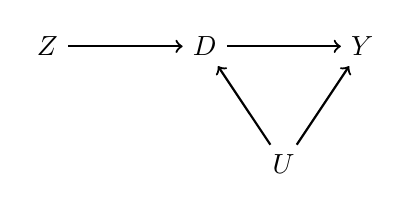
\begin{tikzpicture}[->, node distance=2cm, thick]
    % Nodes
    \node (Z) at (0, 0) {\(Z\)};
    \node (D) at (2, 0) {\(D\)};
    \node (Y) at (4, 0) {\(Y\)};
    \node (U) at (3, -1.5) {\(U\)};

    % Arrows
    \draw[->] (Z) -- (D);
    \draw[->] (D) -- (Y);   
    \draw[->] (U) -- (D);
    \draw[->] (U) -- (Y);
\end{tikzpicture}

\text{Among compliers,} Z \to Y \quad \text{and} \quad Z \to D \to Y

\subsection{Classical IV Models}

\textbf{Pre-1990 Parametric Two-Stage Model}

\begin{align*}
    D &= \alpha_0 + \alpha_1 Z + \gamma \tag{A} \\
    Y &= \beta_0 + \beta_1 D + \epsilon \tag{A}
\end{align*}

where \(\epsilon\) and \(\gamma\) are random error terms.

\(Z\) is the IV that follows:
\begin{enumerate}
    \item \text{Relevance:} 
    \[
    \text{Cov}(D, Z) \neq 0 \Rightarrow \alpha_1 \neq 0
    \]
    \item \text{Exclusion Restriction:} \(Z\) does not appear in the second-stage OLS regression, meaning \(Z\) affects \(Y\) only through \(D\).

    \item \text{Unconfoundedness:} 
    \[
    \text{Cov}(Z, Y) = 0 \quad \text{and} \quad \text{Cov}(Z, \epsilon) = 0
    \]
\end{enumerate}

With covariates, the models become:
\begin{align*}
    D &= \alpha_0 + \alpha_1 Z + \alpha_2 X^\top + \gamma \\
    Y &= \beta_0 + \beta_1 D + \beta_2 X^\top + \epsilon
\end{align*}
with the assumptions:
\[
\text{Cov}(Z, \epsilon \mid X) = 0 \quad \text{and} \quad \text{Cov}(Z, \gamma \mid X) = 0
\]
These models are causal if the structural assumptions hold.

\textbf{Structural Equation Model}

\begin{align*}
    D(Z) &= \alpha_0 + \alpha_1 Z + \gamma \tag{B} \\
    Y(Z, D) &= \beta_0 + \beta_1 D + \epsilon \tag{B}
\end{align*}

\textbf{Theorem:} Under the assumptions of SUTVA (Stable Unit Treatment Value Assumption) and the standard IV conditions:
\begin{enumerate}
    \item \text{Relevance:} \(Z \not\perp\!\!\!\perp D\) 
    \item \text{Exclusion Restriction:} \(Y(Z = z, D = d) = Y(D = d)\)
    \item \text{Exchangeable IV:} \(Z \perp\!\!\!\perp (D(Z), Y(Z))\).
\end{enumerate}

The structural equation model (B) implies the observed model (A) under the following assumptions:
\begin{enumerate}
    \item \text{Relevance:} \(\text{Cov}(D, Z) \neq 0\).
    \item \text{Exclusion Restriction:} \(Z\) does not appear in the second-stage OLS regression.
    \item \text{Unconfounded IV:} \(\text{Cov}(Z, Y) = 0\) and \(\text{Cov}(Z, \epsilon) = 0\).
\end{enumerate}

Under the structural model, $\beta_1 = \mathbb{E}[Y(D=1) - Y(D=0)]$. Additionally, under IV, $\beta_1 = \frac{\Cov(Y,Z)}{\Cov(D,Z)}$ (see the "Wald Estimand" from Wald (1940)). The proof of this is as follows:
\begin{proof}
$$D = \alpha_0 + \alpha_1 Z + \nu$$
$$Y = \beta_0 + \beta_1 D + \varepsilon$$
$$\Cov(Y, Z) = \Cov (\beta_0 + \beta_1 D + \varepsilon, Z) = \beta_1 \Cov(D, Z) + \Cov(\varepsilon, Z) = \beta_1 \Cov(D, Z),$$
where in the last step we used the unfounded IV assumption that $\Cov(\varepsilon, Z) = 0$. This gives us the result that (by dividing by $\Cov(D,Z)$):
$$\beta_1 = \frac{\Cov(Y,Z)}{\Cov(D,Z)},$$
which is valid due to relevance since $\Cov(D, Z) \neq 0$.
\end{proof}

\subsubsection{2 Stage Estimate of $\beta_1$}
We now describe the 2-stage least squares estimate of $\beta_1$.

\begin{enumerate}
    \item OLS regress $D \sim Z$. This gives predictions for $\hat{D} = \hat{\alpha}_1 Z$.
    \item OLS regress $Y \sim \hat{D}$, where $\hat{D} = \hat{\alpha}_1Z$. This gives a predicted $\hat{\beta}_1$.
\end{enumerate}

This procedure leads to the following theorem: Under the 2 stage model with $\Cov(D,Z) \neq 0$ and $\Cov(Z,\nu) = \Cov(Z,\varepsilon) = 0$, $\beta_1$ is the coefficient in a population regression of Y on the predicted value from a population regression of $D$ on $Z$.

As a side note, we can also control for covariates by conditioning on them:
$$\beta_1 = \frac{\Cov(Y, Z | X) }{\Cov(D, Z | X)}$$
The two stage approach with covariates becomes:
\begin{enumerate}
    \item OLS regress $D \sim Z, X$, giving predicted $\hat{D} = \hat{\alpha}_1 Z + \hat{\alpha_2}^T X$
    \item OLS regress $Y \sim \hat{D}$ yielding $\hat{\beta}_1$. 

\end{enumerate}
This 2 stage model is easy to implement, but it has strong parametric assumptions, such as linearity, additivity, and constant effects.

Putting all together through the lens of CACE, the average causal effect under compliers is:
$$\beta_1 = \frac{\Cov(Y, Z ) }{\Cov(D, Z )} = \frac{\mathbb{E} [Y | Z = 1] - \mathbb{E} [Y | Z = 0]}{\mathbb{E} [D | Z = 1] - \mathbb{E} [D | Z = 0]} = $$
And the right hand side can be written as (focusing on compliers):
$$= \mathbb{E} [Y(D=1) - Y(D=0) | D(1) > D(0)]$$.
We reiterate that this assumes monotonicity. Additionally, remember that this is untestable, since we cannot observe whether $D_i(1) \geq D_i(0)$.

\subsubsection{Some Practical Considerations}  
In practice, several challenges arise when using preference-based instruments. For example, consider the random assignment of cases to judges (\(Z\)) as an instrument. Here, \(D\) represents whether there is a pre-trial detention, and \(Y\) indicates whether there is a future offense. If \(Z = 1\), it implies that the case was randomly assigned to a harsh judge. However, it is not always possible to assume that \(D_i(1) \geq D_i(0) \ \forall i\), as there may be exceptions. For instance, a harsh judge might show leniency in specific cases due to personal biases or "soft spots" for particular defendants.  

Another practical issue is the limited policy relevance of analyzing effects for unidentified subgroups. Eaton (2010) critiques this approach, stating:  
\begin{quote}  
"This goes beyond the story of looking for an object where the light is strong enough to see. Rather, we have control over the light, but we choose to let it fall where it may and then proclaim that whatever the light illuminates is what we were looking for all along."  
\end{quote}  
This highlights the importance of a structured approach: (1) defining the estimand, (2) ensuring identification, and (3) performing estimation.  

In contrast, a policy-relevant analysis focuses on identifiable subgroups. For example, Kennedy et al. (2019) suggest that predicting which individuals are likely to comply has practical significance. Formally, this can be expressed as:  
\[
\Pr(D(1) > D(0)) = \mathbb{E}[D | X, Z = 1] - \mathbb{E}[D | X, Z = 0].  
\]  
Such an approach ensures that findings align with actionable insights, making them more useful for policymaking.  

\section{Lecture 16: CACE, IV Methods, and Overlap Violations in RDD }{Minji, Hyemin Park, Jiarong Zhou(revisions))}



\subsubsection{Key Definitions:}
\begin{itemize}
    \item \( Z_i \): Treatment assigned to unit \( i \) (1 for treatment, 0 for control).
    \item \( D_i \): Treatment received by unit \( i \) (1 for treatment, 0 for control).
    \item \( Y_i \): Outcome of interest for unit \( i \).
\end{itemize}

\subsection{CACE (Complier Average Causal Effect)}
 The average causal effect of the treatment for individuals who comply with the assigned treatment. 

\subsubsection{Estimation of CACE}
To estimate the CACE under IV assumptions and monotonicity, the formula is given as:


\[
\mathbb{E}\left[ y(D=1) - y(D=0) \mid D(1) > D(0) \right] =
\]
This can be broken down as follows: 
\[
= \frac{\mathbb{E}[Y \mid Z=1] - \mathbb{E}[Y \mid Z=0]}{\mathbb{E}[D \mid Z=1] - \mathbb{E}[D \mid Z=0]}=  \frac{\mathbb{E}\left[ \mathbb{E}[Y \mid X, Z=1] - \mathbb{E}[Y \mid X, Z=0] \right]} {\mathbb{E}\left[ \mathbb{E}[D \mid X, Z=1] - \mathbb{E}[D \mid X, Z=0] \right]}
\]

\subsubsection{How to estimate?}
\begin{itemize}
    \item regression: $\mu_Z(x) = \mathbb{E}[y \mid X, Z=z]$
    \item weighting: $\lambda_Z(x) = \mathbb{E}[D \mid X, Z=z]$
    \item doubly-robust: $e(X) = P(Z=1 \mid X)$
\end{itemize}

\[
\hat{\mu}_2(x) \text{ by regress } y \sim X \mid Z=z
\]
\[
\hat{\lambda}_z(x) \text{ by regress } D \sim X \mid Z=z
\]

\subsection{Estimators}

\begin{itemize}
    \item \textbf{Regression Estimator}:
    \[
\hat{\tau}_{i, reg} = \frac{\sum_{i=1}^{n} \left\{ \hat{\mu}_1(X_i) - \hat{\mu}_0(X_i) \right\}}{\sum_{i=1}^{n} \left\{ \hat{\lambda}_1(X_i) - \hat{\lambda}_0(X_i) \right\}}
\]
    This estimator uses the regression estimates for the potential outcomes and the treatment assignment, providing a way to compute the average causal effect.

    \item \textbf{Inverse Probability Weighting (IPW) Estimator}:
    \[
\hat{\tau}_{i, IPW} = \frac{\sum_{i=1}^{n} \left\{ \frac{Z_i Y_i}{\hat{e}(X_i)} - \frac{(1-Z_i) Y_i}{1 - \hat{e}(X_i)} \right\}}{\sum_{i=1}^{n} \left\{ \frac{Z_i D_i}{\hat{e}(X_i)} - \frac{(1-Z_i) D_i}{1 - \hat{e}(X_i)} \right\}}
\]
    This estimator accounts for bias by weighting the observed outcomes according to the propensity scores.

    \item \textbf{Doubly Robust Estimator}:
  \[
\hat{\tau}_{i, DR} = \frac{\sum_{i=1}^{n} \left\{ \left( \frac{Z_i}{\hat{e}(X_i)} - \frac{(1-Z_i)}{1 - \hat{e}(X_i)} \right) \left( Y_i - \hat{\mu}_z(X_i) \right) + \hat{\mu}_1(X_i) - \hat{\mu}_0(X_i) \right\}}{\sum_{i=1}^{n} \left\{ \left( \frac{Z_i}{\hat{e}(X_i)} - \frac{(1-Z_i)}{1 - \hat{e}(X_i)} \right) \left( D_i - \hat{\lambda}_z(X_i) \right) + \hat{\lambda}(X_i) - \hat{\lambda}_0(X_i) \right\}}
\]
    This estimator combines both regression and weighting approaches, ensuring validity even if one model is misspecified.
\end{itemize}


\subsubsection{Question to Consider}


Should you always use the same covariate to condition on \(D\) and \(Y\)?


\subsubsection{Graphical Interpretation}

The graph outlines the relationships where:

- \(X_1\): Represents measured confounders that affect both \(Z\) and \(Y\).

- \(X_2\): Influences treatment \(D\) but not directly associated with the outcome.

- \(X_3\): Affects outcome \(Y\) without influencing treatment \(D\).

\begin{center}
\begin{tikzpicture}[
  node distance=1.5cm and 2cm, 
  >={Stealth[round]}, 
  thick, 
  observed/.style={fill=white!20, draw=none, font=\large},
  unobserved/.style={draw, circle, minimum size=0.8cm, font=\small},
  square/.style={draw, minimum size=0.8cm, font=\small}
]

% Nodes
\node[observed, square] (X1) at (0,0) {$X_1$ (measured confounder)};
\node[unobserved] (U) at (4,6) {$U$};
\node[observed, square] (X2) at (2,6) {$X_2$};
\node[observed, square] (X3) at (8,6) {$X_3$};
\node[observed] (Z) at (0,4) {$Z$};
\node[observed] (D) at (4,4) {$D$};
\node[observed] (Y) at (8,4) {$Y$};

% Arrows
\draw[->] (X1) -- (Z);
\draw[->] (X2) -- (D);
\draw[->] (X3) -- (Y);
\draw[->] (Z) -- (D);
\draw[->] (D) -- (Y);
\draw[->] (U) -- (D);
\draw[->] (U) -- (Y);
\draw[->] (X1) -- (Y);
\end{tikzpicture}
\end{center}

\begin{itemize}
    \item We should always include \(X_1\) in \(\lambda\) and \(\mu\) regressions to achieve exchangeability.
    \item You can additionally condition on \(X_2\) in \(\lambda\) regress for efficiency.
    \item You can condition on \(X_3\) in \(\mu\) regression for efficiency.
    \item If we condition on \(X_1\), \(X_2\), and \(X_3\) in both \(\lambda\) and \(\mu\), that is fine.
\end{itemize}

\subsubsection{Question}
Which among the regression, IPW, and DR estimators should we use?

\begin{itemize}
    \item If \(e(X)\) is known: Use IPW or DR.
    
    \item If \(e(X)\) is unknown but \(X\) is discrete and low-dimensional, any estimator is good. They are numerically equivalent and optimally efficient.
    
    \item If \(e(X)\) is unknown and \(X\) includes continuous components or is high-dimensional, choose the doubly robust (DR) estimator.
\end{itemize}

\textbf{Additional Explanation:} 

In experimental settings where the instrument propensity \(e(X)\) is known (as determined by the experimental design), using the IPW estimator is generally robust. The robust estimator is also suitable because it utilizes the true \(e(X)\) while also incorporating estimated models.

In cases where \(e(X)\) is unknown but \(X\) is discrete and low-dimensional, we can estimate nuisance functions using empirical distributions, making any estimator effective.

However, when \(e(X)\) is unknown and involves continuous components or is high-dimensional, the doubly robust estimator is preferable. It offers better theoretical properties under milder assumptions, allowing it to perform well even if only some of the nuisance functions are estimated accurately.


\subsection{Beyond the CACE
: Partial Identification of Average Causal Effect}

The average causal effect \(\tau\) is defined as:
\[
\tau = E[Y(D=1)] - E[Y(D=0)]
\]
This represents the expectation if we treated everyone versus treating no one.

Under the monotonicity and exclusion restriction, we can establish bounds:
\[
\tau_L \leq \tau \leq \tau_U
\]

Where:
\[
\tau_L = E[Y | Z=1] - E[Y | (1-D) + D | Z=0]
\]
\[
\tau_U = \tau_L + 1 - E[D | Z=1] + E[D | Z=0]
\]

The length of the bound is determined by the proportion of non-compliers:
\[
1 - (E[D | Z=1] - E[D | Z=0]) = P(D(1) \leq D(0))
\]

This formulation shows that we can partially identify the average causal effect, giving us lower and upper bounds based on observable quantities that can be estimated from the data. 


\newpage
\subsection{Examples of IVs (Instrumental Variables)}

\subsubsection{Challenge: Identifying and Justifying the IV}
One of the challenges with using instrumental variables (IVs) is identifying a valid instrument and justifying its use. The instrument must satisfy key assumptions, including the exclusion restriction, which states that it affects the outcome only through the treatment.

\subsubsection{Experiments with Non-compliance}  
\textbf{Example: Minneapolis Domestic Violence Experiment}  
- \textbf{\(Z\)} (Instrument): The penalty recommendation by officers responding to a domestic violence incident. This recommendation was randomly assigned.  
- \textbf{\(D\)} (Treatment): Whether the officer adhered to the recommended penalty.  
- \textbf{\(Y\)} (Outcome): Whether the individual re-offended.  

This experimental setup involves non-compliance, as officers had the discretion to deviate from the randomly assigned recommendation. In such cases, Instrumental Variable (IV) methods are particularly useful to estimate the causal effect of the recommendation on the likelihood of re-offending.  

\subsubsection{Distance-based Measures}  
\textbf{Example: Family Visitation and Re-offense Rates (Mauro et al., 2008)}  
- \textbf{\(Z\)} (Instrument): The proximity of an inmate’s family to the jail.  
- \textbf{\(D\)} (Treatment): Whether the family visited the inmate.  
- \textbf{\(Y\)} (Outcome): The re-offense rate after release from jail.  

This approach assumes that the distance between the family’s residence and the jail affects the likelihood of visitation but does not directly influence the re-offense rate except through its impact on visitation. By using distance as an instrument, it becomes possible to estimate the causal effect of family visits on post-release behavior.  

\subsubsection{Preference-based Measures}
\textbf{Example :} \\
\textbf{Z} (Instrument): Doctor’s preference for prescribing Paxlovid (an antiviral drug). \\
\textbf{D} (Treatment): Whether the patient was prescribed Paxlovid. \\
\textbf{Y} (Outcome): Potential liver damage as a side effect. \\

The instrument is the variation in doctors' prescribing behavior in this case. Doctors with different preferences might prescribe Paxlovid differently, and this variation can be exploited as an IV to study the effect of Paxlovid on liver damage.

\subsubsection{Time-based Measures (Change in Policy)}
\textbf{Example :} \\
\textbf{Z} (Instrument): Expansion in the mandated reporter law in 2014, which increased the number of people required to report cases of child abuse or neglect. \\
\textbf{D} (Treatment): Whether a child welfare investigation was opened. \\
\textbf{Y} (Outcome): Educational outcomes of children in the family. \\

Here, a policy change creates variation in reporting, which serves as an instrument for the likelihood of child welfare investigations. This variation allows researchers to study the causal effect of an investigation on children's education.

$$X \rightarrow Z \rightarrow D \rightarrow Y$$
Where $X$ are covariates that may affect both the treatment ($D$) and the outcome ($Y$), while $Z$ (the instrument) affects $D$ but only affects $Y$ indirectly through $D$.

\begin{center}
\begin{tikzpicture}[
  node distance=1.5cm and 2cm, 
  >={Stealth[round]}, 
  thick, 
  observed/.style={fill=white!20, draw=none, font=\large},
  unobserved/.style={draw, circle, minimum size=0.8cm, font=\small},
  square/.style={draw, minimum size=0.8cm, font=\small}
]

% Nodes
\node[observed] (Z) {Z};
\node[observed, right=of Z] (D) {D};
\node[observed, right=of D] (Y) {Y};
\node[unobserved, above=of D] (U) {U};
\node[square, below left=of Z] (X) {X};

% Edges
\draw[->] (X) -- (Z);
\draw[->] (X) -- (Y);
\draw[->] (Z) -- (D);
\draw[->] (D) -- (Y);
\draw[->] (U) -- (D);
\draw[->] (U) -- (Y);
\end{tikzpicture}
\end{center}


\subsubsection{Genes: Mendelian Randomization}
\begin{itemize}
    \item \textbf{Mendel's 2nd law:} The law of random assortment states that the inheritance of one trait is independent of other traits.
    \item Mendelian randomization uses genetic variation as an IV to study the causal effects of exposure (e.g., cholesterol levels) on an outcome (e.g., cancer).
\end{itemize}
\textbf{Example :} \\
\textbf{Z} (Instrument): Genes \\
\textbf{D} (Treatment): Cholesterol levels \\
\textbf{Y} (Outcome): Likelihood of developing cancer \\

In Katan (1986), apolipoprotein E genes were used as an instrument to study the effect of cholesterol levels on cancer risk. The assumption here is that genes affect cholesterol levels but do not directly affect cancer, satisfying the exclusion restriction.

\begin{center}
\begin{tikzpicture}[
  node distance=1.5cm and 2cm,
  >={Stealth[round]}, 
  thick, 
  observed/.style={draw=none, font=\small},
  unobserved/.style={draw, circle, minimum size=1cm, font=\small}
]

% Nodes
\node[observed] (G1) {$G_1$};
\node[observed, below=0.7cm of G1] (G2) {$G_2$};
\node[observed, below=0.7cm of G2] (Gdots) {$\vdots$};
\node[observed, below=0.7cm of Gdots] (Gp) {$G_p$};
\node[observed, right=of Gdots, xshift=1cm] (D) {$D$};
\node[unobserved, above right=of D] (U) {$U$};
\node[observed, right=of D] (Y) {$Y$};

% Edges
\draw[->] (G1) -- (D);
\draw[->] (G2) -- (D);
\draw[->] (Gp) -- (D);
\draw[->] (U) -- (D);
\draw[->] (U) -- (Y);
\draw[->] (D) -- (Y);

\end{tikzpicture}
\end{center}

$$G_1, G_2, \dots, G_p \rightarrow D \rightarrow Y$$
Where $G_1, G_2, \dots, G_p$ represent different genetic variants (instruments), $D$ represents cholesterol levels, and $Y$ represents the outcome (cancer). 

$$G_1, G_2, \dots, G_p \rightarrow U$$
Where $U$ represents unobserved confounders.

\paragraph*{Standard Linear IV Model:}
$$Y = \beta_0 + \beta D + \beta_\mu U + \epsilon_Y$$
$$D = \gamma_0 + \gamma_1 G_1 + \dots + \gamma_p G_p + \gamma_U U + \epsilon_D$$
Here, $Y$ is the outcome, $D$ is the treatment, $G_1, G_2, \dots, G_p$ are the genetic instruments, $U$ is an unobserved confounder, and $\epsilon_Y$ and $\epsilon_D$ are error terms.

\paragraph*{ Reduced Form:}
$$Y = \beta_0 + \beta_D \gamma_0 + \beta_D \gamma_1 G_1 + \dots + \beta_D \gamma_p G_p + (\beta_U + \beta_D \lambda_U) U + \epsilon_Y$$

\paragraph*{Apply Two-Stage Least Squares Estimators to Estimate $\beta$:}
See Chapter 25 of \textit{Ding} for further details.


\subsubsection*{ Critiques of Mendelian Randomization Analyses}
Mendelian Randomization is a powerful tool, but there are several potential issues to consider:
\begin{itemize}
    \item \textbf{SUTVA (Stable Unit Treatment Value Assumption)} or \textbf{target trial emulation} may not be satisfied
    \begin{itemize}
        \item For example, treatment variables like BMI or cholesterol levels may not satisfy SUTVA.
        \item There may be situations where the treatment status of one individual affects the outcome of another, or where the treatment is not well-defined.
    \end{itemize}
    \item \textbf{Exclusion restriction} may be violated
    \begin{itemize}
        \item There may be alternative pathways through which the genes affect the outcome. For example, genes may directly affect cancer development, in addition to affecting cholesterol levels, which would violate the exclusion restriction.
    \end{itemize}
    \item \textbf{Linearity assumption in the IV model} may be violated
    \begin{itemize}
        \item Mendelian Randomization typically assumes a linear relationship between the treatment and the outcome, but in reality, the relationship may be nonlinear.
    \end{itemize}
    \item \textbf{Measurement error} may exist
    \begin{itemize}
        \item The treatment variable (e.g., cholesterol levels) or the outcome variable (e.g., cancer diagnosis) may not be measured accurately, which could lead to biased results.
    \end{itemize}
\end{itemize}


\subsection{Violations of Overlap / Positivity}
\subsubsection{Overlap Condition:}
$$P(0 < e(X) < 1) = 1$$
The overlap or positivity assumption requires that all units have some probability of receiving either treatment or control (i.e., no deterministic treatment assignment). Here. $e(X)$ represents the propensity score.

\subsubsection{Tension between Overlap and Exchangeability:}
There is a tension between the overlap assumption and the exchangeability assumption. As we condition on more covariates to satisfy exchangeability, we may reduce the randomness in the treatment assignment, which can lead to a violation of overlap. \\
\\
\textbf{Example:  Child Welfare Investigation} \\
\textbf{X}: Administrative records, allegations. \\
\textbf{D}: Child welfare investigation \\

In this context, administrative records and the natural language of allegations are used to determine whether a child welfare investigation is opened. Conditioning on these covariates may improve exchangeability but can reduce overlap if these features deterministically affect the treatment decision.


\subsection{Conceptual Challenge: Deterministic Treatment Assignment and Counterfactuals}

In settings where overlap is violated (i.e., units deterministically receive treatment or control), conceptual challenges arise. For instance, what does it mean to consider a counterfactual outcome for a unit that always receives treatment? This raises questions about the definition of potential outcomes for such deterministic units.

To address this, overlap requires that propensity scores be bounded away from 0 and 1:
$$\epsilon < e(X) < 1 - \epsilon$$
where $\epsilon$ is a small positive constant. This boundedness assumption is necessary for many causal inference techniques, particularly in high-dimensional settings.

\subsubsection{Handling Overlap Violations: Trimming}
One common approach to handle overlap violations is trimming, where observations with extreme propensity scores are removed from the analysis. The downside is that this changes the estimand, meaning we are no longer estimating the causal effect for the entire population but rather for a subset where overlap holds.

\subsection{Regression Discontinuity Design (RDD)}

When overlap is violated, an alternative approach is to use a \textbf{regression discontinuity design (RDD)}. RDD is useful in settings with a threshold-based decision rule, where the decision threshold can be considered somewhat arbitrary. By examining outcomes near the threshold, we can assume that the groups on either side are exchangeable, and we can estimate causal effects by comparing outcomes just above and below the threshold.

\subsubsection{Example: COVID-19 Treatment and Oxygen Levels}

Consider a new antiviral COVID-19 treatment. We want to measure its impact on oxygen levels (a continuous outcome) one week after treatment. During the pandemic, this treatment was restricted to high-risk patients, specifically those aged 65 and older.

\begin{itemize}
    \item \textbf{Treatment Group}: Patients aged 65 and older.
    \item \textbf{Control Group}: Patients under 65.
\end{itemize}

Since there is no randomness in who receives the treatment (i.e., there is no overlap), we cannot apply typical causal inference methods. However, we can use RDD by assuming continuity of the outcome regression functions around the threshold (age 65).

\subsubsection{Assumptions for RDD:}
The key assumption in RDD is that the outcome regression functions are continuous at the threshold:
$$\lim_{X \to 65^-} E[Y | X] = \lim_{X \to 65^+} E[Y | X]$$
where $X$ is the age variable. Under this assumption, the difference in outcomes around age 65 can be attributed to the causal effect of the treatment.

\textbf{Interpretation}
The causal effect of the treatment is estimated by the difference in the observed means just above and below the threshold:
$$\text{Causal Effect} = E[Y | X = 65^+] - E[Y | X = 65^-]$$

In this example, we would observe oxygen levels (Y) for patients just below 65 (control group) and just above 65 (treatment group) and interpret the difference in means as the causal effect of the COVID-19 treatment.

\subsection*{Next Class}
How to implement a regression discontinuity analysis in practice. \\
Reminder: there is a midterm exam scheduled for next Tuesday.

\section{Lecture 17: Sharp Regression Discontinuity Design (RDD)}{Carlos Guirado, Stella Jia, Kayla Sim(revisions)}

\subsection{Regression Discontinuity Design (RDD)}

\subsubsection{Introduction and Motivating Example}

In the last lecture, Regression Discontinuity (RD) was introduced through a COVID treatment example:
\begin{itemize}
    \item Treatment (D): New antiviral COVID treatment
    \item Outcome (Y): Patient oxygen levels
    \item Running variable (X): Age
    \item Policy: Treatment restricted to those 65 and older
\end{itemize}

This creates a sharp discontinuity in treatment probability:
\[P(D=1|X \geq 65) = 1\]
\[P(D=1|X < 65) = 0\]

\subsubsection{Exchangeability in RD}

A key feature of RD is that exchangeability holds by design. This can be understood by examining the causal structure:

\begin{enumerate}
    \item The running variable X (age) determines treatment D:
    \[D = \mathbf{1}[X \geq x_0]\]
    
    \item Traditional settings require:
    \begin{itemize}
        \item Both exchangeability and overlap
        \item D as a function of X and other variables V:
        \[D = f(X,V)\]
        \item V affects D but not Y for overlap to hold
    \end{itemize}
    
    \item In sharp RD:
    \begin{itemize}
        \item Overlap does not hold
        \item D is determined solely by X (i.e. deterministic)
        \item Conditioning on X eliminates all unobserved confounding
        \item Exchangeability holds automatically due to treatment assignment mechanism
    \end{itemize}
\end{enumerate}

\subsubsection{Examples of RD in Practice}

\begin{enumerate}
    \item Thistlethwaite \& Campbell (1960) - First RD study:
    \begin{itemize}
        \item D: Certificate of merit
        \item Treatment rule: \[D = \mathbf{1}[\text{test score} \geq 10.5]\]
        \item Y: Plans for graduate study and scientific research
        \item Demonstrated how seemingly arbitrary cutoffs can be leveraged for causal inference
    \end{itemize}

    \item Carpenter \& Dobkin (2009):
    \begin{itemize}
        \item D: Legal drinking status
        \item Treatment rule: \[D = \mathbf{1}[\text{age} \geq 21]\]
        \item Y: Death outcomes
        \item Examined different types of mortality:
        \begin{itemize}
            \item Overall mortality
            \item Alcohol-related deaths
            \item External vs. internal causes of death
        \end{itemize}
    \end{itemize}
\end{enumerate}

\subsubsection{Formal Treatment and Identification}

RD identifies the local average treatment effect at the threshold:
\[\tau(x_0) = \mathbb{E}[Y(1) - Y(0)|X=x_0]\]

The identification strategy differs from traditional approaches:

\begin{enumerate}
    \item For treated potential outcome:
    \[\mathbb{E}[Y(1)|X=x_0] = \lim_{\epsilon \to 0^+} \mathbb{E}[Y(1)|X=x_0+\epsilon]\]
    \[= \lim_{\epsilon \to 0^+} \mathbb{E}[Y(1)|D=1, X=x_0+\epsilon]\]
    \[= \lim_{\epsilon \to 0^+} \mathbb{E}[Y|D=1, X=x_0+\epsilon]\]

    \item For control potential outcome:
    \[\mathbb{E}[Y(0)|X=x_0] = \lim_{\epsilon \to 0^+} \mathbb{E}[Y|D=0, X=x_0-\epsilon]\]

    \item The treatment effect:
    \[\tau(x_0) = \lim_{\epsilon \to 0^+} \mathbb{E}[Y|D=1, X=x_0+\epsilon] - \lim_{\epsilon \to 0^+} \mathbb{E}[Y|D=0, X=x_0-\epsilon]\]
\end{enumerate}

\subsubsection{Local Linear Regression Approach}

Implementation typically uses local linear regression:

\begin{enumerate}
    \item Basic procedure:
    \begin{itemize}
        \item Select observations near threshold $x=x_0$
        \item Fit separate linear models on each side of the threshold
        \item Compare fitted values at threshold
    \end{itemize}

    \item Critical bandwidth choice considerations:
    \begin{itemize}
        \item Too small (e.g., 1 day from threshold):
        \begin{itemize}
            \item Few data points
            \item High variance in estimates
        \end{itemize}
        \item Too large (e.g., 2 years from threshold):
        \begin{itemize}
            \item Bias from comparing non-exchangeable individuals
            \item Other factors may vary over wider window
        \end{itemize}
    \end{itemize}

    \item Practical recommendations:
    \begin{itemize}
        \item Report estimates for multiple bandwidths
        \item Include confidence intervals
        \item Use \texttt{rdrobust} package in R
        \item Consider covariate adjustment for wider bandwidths
    \end{itemize}
\end{enumerate}

\subsubsection{Limitations and Potential Problems}

\begin{enumerate}
    \item Data sensitivity:
    \begin{itemize}
        \item Results vulnerable to leverage points near cutoff
        \item Individual observations can heavily influence slope estimates
    \end{itemize}

    \item Continuity assumption:
    \begin{itemize}
        \item Requires continuity in potential outcome regression functions
        \item Not directly testable as counterfactual outcomes unobservable
        \item $\mu_1(x)$ and $\mu_0(x)$ not fully observable
    \end{itemize}

    \item Multiple threshold effects:
    \begin{itemize}
        \item Other treatments/policies may change at threshold
        \item Example: Medicare eligibility at age 65
        \item Complicates isolation of specific treatment effect
        \item May affect interpretation of results
    \end{itemize}

    \item Bandwidth selection challenges:
    \begin{itemize}
        \item Tradeoff between bias and variance
        \item Results may be sensitive to choice
        \item Need to demonstrate robustness across choices
    \end{itemize}
\end{enumerate}

\subsubsection{Comparison to Traditional Experiments}

When considering RD designs, it's useful to think about the ideal experiment:
\begin{itemize}
    \item Traditional experiment might randomize treatment directly
    \item RD approximates experiment around threshold
    \item Treatment effect identified only for subpopulation near threshold
    \item Requires additional assumptions for broader generalization
\end{itemize}

\subsection*{Class Survey}
This lecture was shorter than usual as students were given time to complete a course evaluation survey.

\subsection*{Next Class}
Fuzzy regression  discontinuity design.

\section{Lecture 18: Fuzzy Regression Discontinuity Design (RDD)}{Harish Srinivasan, Aditya Vunnum, Simon Cha, Kayla Sim (revisions)}

\subsection{Wrapping Up Regression Discontinuity}

\subsubsection{Sharp RDD Recap}

In the previous lecture, we explored the concept of Sharp Regression Discontinuity Design (RDD), which uses a strict cutoff point in the running variable to determine treatment assignment. 
\[D = \mathbf{1}[X \geq x_0]\]

A key example was a COVID treatment policy:
\begin{itemize}
    \item \textbf{Treatment (D)}: Administration of a new antiviral COVID treatment.
    \item \textbf{Outcome (Y)}: Patient oxygen levels.
    \item \textbf{Running Variable (X)}: Age.
    \item \textbf{Policy Rule}: Treatment was provided only to patients aged 65 and older.
\end{itemize}

This setup created a sharp discontinuity in treatment probability:
\[
P(D=1|X \geq 65) = 1, \quad P(D=1|X < 65) = 0
\]
The sharp cutoff at age 65 made treatment assignment deterministic based on age alone, allowing for causal inference by comparing outcomes immediately on either side of the threshold.

\textbf{Exchangeability} holds by design in Sharp RDD. Since treatment is fully determined by the running variable, conditioning on the running variable (age in this case) controls for unobserved confounding. This setup does not require overlap between treatment and control groups, as assignment is non-random and based purely on the cutoff.

\subsubsection{Transition to Fuzzy RDD}

In practice, strict cutoff rules are not always feasible, leading to the development of Fuzzy RDD. In Fuzzy RDD, the probability of treatment changes at the threshold, but treatment is not strictly assigned based on the cutoff. Instead, the threshold increases the likelihood of treatment, introducing ``fuzziness."

\subsection{Fuzzy Regression Discontinuity Design (RDD)}

\subsubsection{Introduction to Fuzzy RDD}

Fuzzy RDD relaxes the strict assignment of treatment, allowing for a probabilistic jump in treatment assignment at the threshold. This is useful in settings where the treatment may be recommended but not enforced strictly based on the running variable.

Today’s example uses a treatment indicator \( Z \) defined as:
\[
Z = \mathbf{1}[X \geq x_0]
\]
where \( X \) is the running variable and \( x_0 \) is the cutoff. With Fuzzy RDD, the probability of treatment \( P(D=1 | X=x) \) has a jump at \( X = x_0 \), but treatment is not assigned deterministically.

\subsubsection{Examples of Fuzzy RDD in Practice}

\paragraph{Example 1: College Admissions}
\begin{itemize}
    \item A fuzzy cutoff is applied with SAT scores around 1300.
    \item Colleges may admit students who score below the threshold if they excel in other areas, and may reject students above the threshold if their grades are poor.
\end{itemize}

\paragraph{Example 2: Eligibility for Social Assistance}
\begin{itemize}
    \item A social assistance program uses a predicted income threshold \( X \leq x_0 \) to determine eligibility.
    \item Not all eligible families enroll, and other eligibility criteria may apply.
\end{itemize}

The estimand for the local complier average causal effect in this setup is:
\[
\tau_c(x_0) = \mathbb{E} \left[ Y(D=1) - Y(D=0) \mid D(1) > D(0), X = x_0 \right]
\]

\subsection{Theorem for Fuzzy RDD}

Under the following conditions:
\begin{enumerate}
    \item Monotonicity: \(D(1) \geq D(0)\)
    \item Exclusion restriction: \((Y(Z=z, D=d) = Y(D=d))\)
\end{enumerate}
the local complier average causal effect is given by:
\[
\tau_{c}(x_0) = \frac{\mathbb{E} \left[ Y(D=1) - Y(D=0) \mid X = x_0 \right]}{\mathbb{E} \left[ D(1) - D(0) \mid X = x_0 \right]}
\]

Under continuity conditions, and if \( P(D=1|X=x) \) has a jump at \( x_0 \), then \( \tau_c(x_0) \) is identified as:
\[
\tau_c(x_0) = (\lim_{\epsilon \to 0^+} \mathbb{E}[Y|Z=1, X=x_0+\epsilon] - \lim_{\epsilon \to 0^+} \mathbb{E}[Y|Z=0, X=x_0-\epsilon])
\]
\[
\div (\lim_{\epsilon \to 0^+} \mathbb{E}[D|Z=1, X=x_0+\epsilon] - \lim_{\epsilon \to 0^+} \mathbb{E}[D|Z=0, X=x_0-\epsilon])
\]

For more details, see Chapter 24 of \emph{Imbens \& Lemieux (2008)}.

\subsection{Causal Inference under Unobserved Confounding}

\subsubsection{Sensitivity to Ignorability Assumption}

It's essential to understand how sensitive results are to the assumption of ignorability.

\paragraph{Example: Smoking and Lung Cancer}
\begin{itemize}
    \item Doll and Hill (1950) found that the risk ratio for smoking on lung cancer was 9.
    \item However, Fisher (1957) proposed that a common genetic cause might be responsible for both smoking and lung cancer.
\end{itemize}

The sensitivity parameter describes the strength of this unobserved confounding.

\subsubsection{Sensitivity Parameters}

For binary \(Y\) and binary \(U\):
\[
Z \not\!\perp\!\!\!\perp \{Y(1), Y(0)\} \mid X
\]
\[
Z \ind \{Y(1), Y(0)\} \mid X, U
\]

Define two sensitivity parameters:
\begin{enumerate}
    \item \(\text{RR}_{ZU|X} = \frac{P(U=1 \mid Z=1, X=x)}{P(U=1 \mid Z=0, X=x)}\)
    \item \(\text{RR}_{YU|X} = \frac{P(Y=1 \mid U=1, X=x)}{P(Y=1 \mid U=0, X=x)}\)
\end{enumerate}

\subsubsection{Observed Risk Ratio}

The observed risk ratio is given by:
\[
\text{RR}_{ZY|X}^{obs} = \frac{P(Y=1|Z=1, X=x)}{P(Y=1|Z=0, X=x)}
\]
Under unmeasured confounding, the true risk ratio differs:
\[
\text{RR}_{ZY|X}^{true} = \frac{P(Y(1)=1|X=x)}{P(Y(0)=1|X=x)}
\]

\subsubsection{Theorem for Sensitivity Analysis}

The observed risk ratio under unobserved confounding is bounded by:
\[
\text{RR}_{ZY|X}^{\text{obs}} \leq \frac{\text{RR}_{ZU|X} \cdot \text{RR}_{YU|X}}{\text{RR}_{ZU|X} + \text{RR}_{YU|X} - 1}
\]

Assuming \( Z \perp Y \mid (X, U) \) and, without loss of generality, that:
\[
\text{RR}_{ZY|X}^{\text{obs}} > 1, \quad \text{RR}_{ZU|X} > 1, \quad \text{RR}_{YU|X} > 1.
\]

\subsubsection{Implications of the Theorem}

The theorem implies that:
\[
\text{RR}_{ZU|X} \geq \text{RR}_{ZY|X}^{\text{obs}}
\]
\[
\text{RR}_{YU|X} \geq \text{RR}_{ZY|X}^{\text{obs}}
\]
This is known as the \textbf{Cornfield inequality}. 

To explain away the observed relative risk, both confounding measures \(\text{RR}_{ZU|X}\) and \(\text{RR}_{YU|X}\) must be at least as large as \(\text{RR}_{ZY|X}^{\text{obs}}\).


\subsubsection{Bounding the Average Causal Effect without Sensitivity Parameters}

Assume \( \underline{Y} \leq Y \leq \overline{Y} \), meaning the outcome is bounded. The average causal effect can be bounded as:
\[
\tau = \mathbb{E}[Y(1) - Y(0)]
\]
\[
\tau \leq \overline{Y} - \underline{Y}
\]

If \(\tau\) is partially identified, multiple values of \(\tau\) are compatible with the observed data distribution, as discussed in \emph{Manski (1990, 2003)}. However, bounds typically cover zero.

More informative bounds can be obtained when combined with other assumptions, such as monotonicity:
\[
Y(1) \geq Y(0) \Rightarrow \epsilon_0 \leq 0
\]

Define the sensitivity parameters:
\[
\epsilon_1(X) = \frac{\mathbb{E}[Y(1) \mid Z=1, X]}{\mathbb{E}[Y(1) \mid Z=0, X]}
\]
\[
\epsilon_0(X) = \frac{\mathbb{E}[Y(0) \mid Z=1, X]}{\mathbb{E}[Y(0) \mid Z=0, X]}
\]

\subsubsection{Theorem}



\[
\mathbb{E}[Y(1) \mid Z=0] = \mathbb{E} \left[ \frac{\mathbb{E}[Y \mid Z=1, X]}{\epsilon_1(X)} \mid Z=0 \right]
\]
\[
\mathbb{E}[Y(0) \mid Z=1] = \mathbb{E} \left[ \mathbb{E}[Y \mid Z=0, X] \epsilon_0(X) \mid Z=1 \right]
\]

where \( \epsilon_1(X) \) and \( \epsilon_0(X) \) are sensitivity parameters.





\subsection{Estimators}


\subsubsection{Estimators}

Define the following estimators:

1. \(\hat{\tau}_{\text{ht}}\):
\[
\hat{\tau}_{\text{ht}} = \frac{1}{n} \sum_{i=1}^n \left( \frac{Z_i Y_i \left( \hat{e}(X_i) + (1 - \hat{e}(X_i)) / \epsilon_1(X_i) \right)}{\hat{e}(X_i)} - \frac{\hat{e}(X_i) \epsilon_0(X_i) + (1 - \hat{e}(X_i))(1 - Z_i) Y_i}{1 - \hat{e}(X_i)} \right)
\]


2. \(\hat{\tau}_{\text{haj}}\):
\[
\hat{\tau}_{\text{haj}} = \frac{\sum_{i=1}^n \frac{\hat{e}(X_i) \epsilon_0(X_i) + (1 - \hat{e}(X_i))(1 - Z_i) Y_i}{1 - \hat{e}(X_i)}}{\sum_{i=1}^n \frac{1 - Z_i}{1 - \hat{e}(X_i)}}
\]



3. \(\hat{\tau}_{\text{OR}}\):
\[
\hat{\tau}_{\text{OR}} = \hat{\tau}_{\text{HT}} - \frac{1}{n} \sum_{i=1}^n \left( Z_i - \hat{e}(X_i) \right) \left( \frac{\hat{\mu}_1(X_i)}{\hat{e}(X_i) \epsilon_1(X_i)} + \frac{\hat{\mu}_0(X_i) \epsilon_0(X_i)}{1 - \hat{e}(X_i)} \right)
\]



\subsection{Calibrating Sensitivity Parameters Using Observed Covariates}

Using a leave-one-out approach:
\[
\epsilon_z(X_{-j}) = \frac{\mathbb{E}[Y(z) | Z=1, X_{-j}]}{\mathbb{E}[Y(z) | Z=0, X_{-j}]}
\]

Under \(Z \perp Y(z) \mid X\), we have:
\[
\epsilon_z(X) = \exp(\alpha z + \beta^T z)
\]

\section{Lecture 19: Sensitivity Analysis}{Isabel Moreno,
Jane Chen,
Xuanlin Mao, \\ Kayla Sim(revisions)}

\subsection{Strategies for causal inference under unobserved confounding}

\subsubsection{Cornfield-style inequalities and Manski-style bounds: bound estimand using outcome bounds - recap}

In the previous lecture, the first two strategies were introduced:

\begin{itemize}
    \item 1. \textbf{Cornfield-style} inequalities provide a way to bound the \emph{relative risk} (RR) in the presence of unobserved confounding variables. These inequalities express a relationship between observed treatment effects and the potential impact of confounders.
\[RR^{obs}_{zy|x}\leq  min(RR_{zu|x},RR_{uy|x})\]

\item 2. \textbf{Manski-style bounds} are used to bound the estimand by placing bounds on the outcomes. These can be represented as:
\[
\underline{y} \leq y \leq \overline{y}
\]
For treatment outcomes:
\begin{itemize}
\[
\underline{y} \leq E[y(0) | z=1] \leq \overline{y}
\]
\[
\underline{y} \leq E[y(1) | z=0] \leq \overline{y}
\]

\end{itemize}
\end{itemize}

\subsection{Rosenbaum-Style Sensitivity Analysis}

Rosenbaum (1987) introduced a sensitivity analysis for one-to-one matched observational studies to test the sharp null hypothesis of no individual treatment effect.

\textbf{Example:} Consider the following variables:
\begin{itemize}
    \item \( Z \) = in-class lecture attendance (treatment),
    \item \( Y \) = grade (outcome),
    \item \( X \) = graduate student, statistics concentration (covariate),
    \item \( U \) = studiousness, passion for the subject, etc. (unobserved confounder).
\end{itemize}

The sharp null hypothesis asserts that attending the lecture in person has no effect on anyone’s grade.

\subsubsection{Notation and Setup}

Let \((i, j)\) index pair \(j\) in unit \(i\), where \( i = 1, 2, \dots, n \) and \( j = 1, 2 \).

\[
H_0^f: Y_{ij}(1) = Y_{ij}(0) \quad \text{for} \quad i = 1, 2, \dots, n, \quad j = 1, 2
\]
Let:
\[
z_{ij} = \text{treatment assigned to unit } (i,j),
\]
\[
e_{ij} = P(Z_{ij} = 1 | X_i, Y_{ij}(1), Y_{ij}(0)) \quad \text{(true propensity score)},
\]
\[
X_i = \text{covariates of the } i \text{th pair (assume perfect matching)}.
\]
\[
O_{ij} = \frac{e_{ij}}{1 - e_{ij}} \quad \text{(odds of treatment for unit } (i, j)\text{)}.
\]

\subsubsection{Rosenbaum Sensitivity Analysis Model}

The sensitivity model is defined as:
\[
\frac{\sigma_{i1}}{\sigma_{i2}} \leq \Gamma, \quad \frac{\sigma_{i2}}{\sigma_{i1}} \leq \Gamma \quad \text{for} \quad i = 1, 2, \dots, n,
\]
which is equivalent to:
\[
\frac{1}{1 + \Gamma} \leq \pi_{i1} \leq \frac{\Gamma}{1 + \Gamma} \quad \text{for} \quad i = 1, 2, \dots, n,
\]

Where: 
\[\pi_{i1}=P(Z_{i1}=1|X_i, Z_{i1}+Z_{i2}=1, Y_{i1}(0), Y_{i2}(0), Y_{i1}(1), Y_{i2}(1))\]

\[\pi_{i1}=\frac{e_{i1}(1-e_{i2})}{e_{i1}(1-e_{i2})+e_{i2}(1-e_{i1})}\]

where \(\pi_{i1}\) is the probability of receiving treatment \(Z_{i1} = 1\), conditioned on covariates and potential outcomes.

If there is no unobserved confounding, we have:
\[
e_{ij} = P(Z_{ij} = 1 | X_i),
\]
which leads to:
\[
e_{i1} = e_{i2}, \quad \pi_{i1} = \frac{1}{2}, \quad \Gamma = 1 = \frac{\sigma_{i1}}{\sigma_{i2}}.
\]

\subsubsection{Testing the Sharp Null Hypothesis}

To test the sharp null hypothesis, we examine the within-pair sign. Under the null hypothesis (\(H_0^f\)), the distribution of the sign\(S_i\) follows a Bernoulli(1/2):

Let 
\[\hat{\tau_i} = (2Z_{ij} - 1)(Y_{i1}- Y_{i2})\]

\[
S_i \sim \text{Bernoulli}(\pi_{i1}),
\]
where the worst-case scenario under the Rosenbaum model is:
\[
S_i \sim \text{Bernoulli}\left(\frac{\Gamma}{1 + \Gamma}\right).
\]

\paragraph{Test Statistics}

Two common test statistics are used in matching:
\begin{itemize}
    \item 1. \textbf{Sign Statistic:} 
   \[
   T = \sum_{i=1}^n S_i.
   \]
   \item  2. \textbf{Wilcoxon Signed-Rank Statistic:} 
   \[
   T = \sum_{i=1}^n S_i R_i,
   \]
   where \(R_i\) is the rank of the absolute value of \(T_i\).
\end{itemize}

\textbf{Generalization:}
   \[T = \sum S_i q_i\]
   
The distribution of \(T\) has the following properties:
\[
E_\Gamma(T) = \frac{\Gamma}{1 + \Gamma} \sum_{i=1}^n q_i,
\]
\[
\text{Var}_\Gamma(T) = \frac{\Gamma}{(1 + \Gamma)^2} \sum_{i=1}^n q_i^2.
\]
The normal approximation of \(T\) is given by:
\[
\frac{T - \frac{\Gamma}{1 + \Gamma} \sum_{i=1}^n q_i}{\sqrt{\frac{\Gamma}{(1 + \Gamma)^2} \sum_{i=1}^n q_i^2}} \to N(0, 1).
\]

\subsubsection{Generalizing the Rosenbaum Model Beyond 1-1 Matching}

In the general model, the assumption is:
\[
Z \not\perp\!\!\!\perp (Y(1), Y(0)) | X, \quad Z \perp\!\!\!\perp (Y(1), Y(0)) | X, U.
\]
The odds ratio model becomes:
\[
\frac{1}{\Gamma} \leq \frac{\text{odds}(Z=1 | X, U = u)}{\text{odds}(Z=1 | X, U = u')} \leq \Gamma \quad \text{for any} \quad u, u'.
\]

Where \(\Gamma\) is a measure of how far we are from the perfect unconfounded experiment

The marginal sensitivity model is:
\[
\frac{1}{\Gamma} \leq \frac{\text{odds}(Z=1 | X, U)}{\text{odds}(Z=1 | X)} \leq \Gamma,
\]
which is equivalent to:
\[
\frac{1}{\Gamma} \leq \frac{\frac{P(Z=1 | X, U=u)}{P(Z=0 | X, U=u)}}{\frac{P(Z=1 | X)}{P(Z=0 | X)}} \leq \Gamma.
\]

Once we specify \(\Gamma\), we can partially identify our estimand under the marginal sensitivity model (MSM) and proceed with the estimation of the partially identified target.

\section{Lecture 20: Principal Stratification and Mediation}{Yixin Feng, Keira Chiu, Allie Huang, Fangyuan Li(revisions)}
\subsection*{Announcements:}
\begin{itemize}
    \item No lecture Thursday - BSTARS 1-5
    \item 256: submit video on Gradescope
    \item Project signups
    \item Midterm grades released
\end{itemize}

\subsection*{Challenge example:}
\begin{itemize}
    \item Officers are as likely to shoot a white person they stop as a black person (Fryer 2019)
    \item Officers are more likely to use unjustified force on black people
    \item Example of post-treatment bias:
    \begin{itemize}
        \item Treatment: race
        \item Post-treatment variable: stop
        \item Outcome: shoot
    \end{itemize}
\end{itemize}

\subsection*{Post-treatment Variables}
\begin{itemize}
    \item \textbf{Police bias:}
    \begin{itemize}
        \item $Y$: use of force
        \item $Z$: race of driver/pedestrian
        \item $M$: stopped driver/pedestrian
    \end{itemize}
    \item \textbf{Job training:}
    \begin{itemize}
        \item $Z$: job training
        \item $Y$: wage
        \item $M$: employment status
    \end{itemize}
    \item \textbf{Clinical trial:}
    \begin{itemize}
        \item $Z$: HIV treatment
        \item $Y$: 30-year survival
        \item $M$: surrogate endpoints
        \item e.g., CD4 cell counts
    \end{itemize}
\end{itemize}

\subsection*{Completely Randomized Experiment}
\[
Z = \{ Y(0), Y(1), M(0), M(1) \}
\]

\textbf{Goal: Compare $P(Y(1) | M = m)$ vs $P(Y(0) | M = m)$}

Can we use $P(Y|Z=1, M=m)$ vs $P(Y|Z=0, M=m)$?

By CRE:
\[
P(Y|Z=1, M=m) = P(Y(1)|Z=1, M(1) = m) = P(Y(1)| M(1) = m)
\]
\[
P(Y|Z=0, M=m) = P(Y(0)|Z=0, M(0) = m) = P(Y(0)| M(0) = m)
\]
In the challenge example, comparing \( P(Y \mid Z=1, M=m) \) and \( P(Y \mid Z=0, M=m) \) involves two different populations. Specifically, \( Y(1) \) represents the outcome for all black drivers, while \( M(1) = 1 \) corresponds to black drivers who are stopped. Similarly, \( Y(0) \) represents the outcome for all white drivers, and \( M(0) = 0 \) corresponds to white drivers who are stopped. Since these comparisons condition on two completely different populations, it is not possible to determine whether the causal effect is due to the causal relationship between \( Y \) and \( Z \), or if it arises because we are not comparing equivalent groups. Comparing causal effects using different populations can introduce bias, as the comparisons may not accurately reflect the true causal relationships.


\textbf{Another example:} truncation by death \newline
    \quad \( Z \): severe disease treatment \newline
    \( \quad Y \): quality of life \newline
    \( \quad M \): survival status \newline
    
Suppose treatment affects survival status, so treatment can save more weak patients than control. 
\[P(Y(1)|M(1)=1) \text{ vs } P(Y(0)|M(0)=1)\]
where the first includes weaker patients, and the second does not.

\subsection{Principal Stratification: conditioning on potential}

\subsubsection{Values of post-treatment variables (Frangakis and Rubin 2002):}

Goal: compare 
\(P(Y(1)|M(1)=m_1, M(0) = m_0) \text{ vs } P(Y(0)|M(1)=m_1, M(0) = m_0)\) for some \(m_1, m_0\).

\begin{itemize}
    \item \(M(1)\), \(M(0)\) are pre-treatment covariates:
    \item Principal strata defined by potential values of post-treatment variable

\end{itemize}

Ex: Binary M

Principal strata, severe disease example:

\(M(1)=1\), \(M(0)=1\) survive always \newline
\(M(1)=1\), \(M(0)=0\) need treatment to survive \newline
\(M(1)=0\), \(M(0)=1\) harmed by treatment \newline
\(M(1)=0\), \(M(0)=0\) doomed \newline

\textbf{Define:}
\[\tau(m_1, m_0) = E[Y(1) - Y(0) \text{ }| \text{ } M(1) = m_1, M(0) = m_0]\] as the Principal Stratification Average Causal Effect for subgroup with \(M(1) = m_1\) and \(M(0) = m_0\).

For binary M, we have four effects:
\[\tau(1, 1) = E[Y(1) - Y(0) \text{ }| \text{ } M(1) = 1, M(0) = 1]\]
\[\tau(1, 0) = E[Y(1) - Y(0) \text{ }| \text{ } M(1) = 1, M(0) = 0]\]
\[\tau(0, 1) = E[Y(1) - Y(0) \text{ }| \text{ } M(1) = 0, M(0) = 1]\]
\[\tau(0, 0) = E[Y(1) - Y(0) \text{ }| \text{ } M(1) = 0, M(0) = 0]\]
where \(\tau(1, 1)\) and \(\tau(0,0)\) are measures of dissociative effects, and \(\tau(1, 0)\) and \(\tau(0,1)\) are measures of associative effects.

\textbf{Example:} experiment with noncompliance \newline
    \( Z \): treatment assigned \newline
    \( Y \): treatment received (we used D for this previously) \newline
    \( M \): outcome

\begin{center}
\begin{tikzpicture}[
  node distance=1.5cm and 2cm, 
  >={Stealth[round]}, 
  thick, 
  observed/.style={fill=white!20, draw=none, font=\large},
  unobserved/.style={draw, circle, minimum size=0.8cm, font=\small},
  square/.style={draw, minimum size=0.8cm, font=\small}
]

% Nodes
\node[observed] (M) {M};
\node[observed, right=of M] (Y) {Y};
\node[unobserved, above=of M] (U) {U};
\node[observed, below left=of M] (Z) {Z};

% Edges
\draw[->] (Z) -- (M);
\draw[->] (Z) -- (Y);
\draw[->] (M) -- (Y);
\draw[->] (U) -- (M);
\draw[->] (U) -- (Y);
\end{tikzpicture}
\end{center}

\(\tau(1,1)\) always takers effect \newline
\(\tau(1,1)\) compliers effect \newline
\(\tau(1,1)\) defiers effect \newline
\(\tau(1,1)\) never takers effect \newline

\textbf{Example:} severe disease
    \begin{itemize}
        \item \(Y(M=0)\) is not well defined (\(Y\) is quality of life).
        \item Only \(\tau(1,1)\) is well defined.
        \begin{itemize}
            \item Survivor average causal effect (Rubin 2006) 
        \end{itemize}

    \end{itemize}

\textbf{Example: Unemployment}
\begin{itemize}
    \item \( Y \): wage
    \item \( Z \): job training
    \item \( M \): employment status
\end{itemize}

\textbf{Note:} Only \( \tau(1, 1) \) is well-defined.

\textbf{Example: Clinical Trial}
\begin{itemize}
    \item A good surrogate meets two criteria:
    \begin{enumerate}
        \item If treatment doesn’t affect the surrogate, then it doesn’t affect the outcome (\textbf{causal necessity}).
        \item If treatment affects the surrogate, then it affects the outcome too (\textbf{causal sufficiency}).
    \end{enumerate}
    \item \textbf{Causal necessity} requires:
    \[
    \tau(1,1) \text{ and } \tau(0,0) = 0.
    \]
    \item \textbf{Causal sufficiency} requires:
    \[
    \tau(1,0) \text{ and } \tau(0,1) \neq 0.
    \]
\end{itemize}

\subsection{Identification of $\tau(m_1, m_0)$}
To identify \( \tau(m_1, m_0) = E[Y(1) - Y(0) \mid M(1) = m_1, M(0) = m_0] \), we rely on the following assumptions:

\subsubsection{Assumptions}
\begin{enumerate}
    \item \textbf{Completely Randomized Experiment (CRE)}: \[ Z \ind \{ Y(1), Y(0), M(1), M(0) \} \]
    \item \textbf{Monotonicity}: \( M(1) \geq M(0) \). \newline
    Example: no defiers in compliance settings.
\end{enumerate}

\subsubsection{Latent Strata Proportions}
Under these assumptions, we can identify the proportions of three latent strata:
\begin{align*}
    \pi(1, 1) &= P(M(1) = 1, M(0) = 1) \\
    \pi(0, 0) &= P(M(1) = 0, M(0) = 0) \\
    \pi(1, 0) &= P(M(1) = 1, M(0) = 0).
\end{align*}
\begin{itemize}
    \item By monotonicity, \( P(M(1) < M(0)) = 0 \).
\end{itemize}

\textbf{Example:} Severe disease and truncation by death. \newline
Only \( \tau(1, 1) \) is well-defined because \( Y(M = 0) \) (e.g., quality of life for non-survivors) is not observable.

\subsubsection{Key Derivations}
To identify \( E[Y(1) \mid M(1) = 1, M(0) = 1] \):
\[
E[Y(1) \mid M(1) = 1, M(0) = 1] = E[Y \mid Z = 1, M = 1] 
\]
However, due to CRE, this cannot directly identify \( E[Y(1) \mid M(1) = 1, M(0) = 1] \), as:
\[
E[Y \mid Z = 1, M = 1] \neq E[Y(1) \mid M(1) = 1, M(0) = 1].
\]

Instead:
\begin{align*}
E[Y(1) \mid M(1) = 1, M(0) = 1] &= E[Y(1) \mid M(1) = 1, M(0) = 1] \cdot P(M(0) = 1 \mid M(1) = 1) \\
&\quad + E[Y(1) \mid M(1) = 1, M(0) = 0] \cdot P(M(0) = 0 \mid M(1) = 1).
\end{align*}

\subsubsection{Partial Identification}
As there is one equation with two unknowns, we cannot point-identify \( E[Y(1) \mid M(1) = 1, M(0) = 0] \). \newline
\textbf{Solution:} Partial identification techniques can provide bounds for the unobservable quantities.

\section{Lecture 21: Guest Lecture about Panel Causal Model}{Lingxi Zhong, Dominic Fannjiang, Fangyuan Li(revisions)}

\subsection*{Note:}

\begin{itemize}
    \item This lecture is a guest lecture offer by professor Avi Feller
\end{itemize}

\subsection*{Panel Data Overview}

\begin{itemize}
    \item \textbf{Cross-sectional data:} Observe a single snapshot in time
        \begin{itemize}
            \item Standard observational data - \textbf{assume away unmeasured confounding.}
            \item Most useful when we have lots of Xs and large N
        \end{itemize}

    \item \textbf{Panel Data:} Observe same units over time. Usually in settings with a small number of units.
        \begin{itemize}
            \item Almost all analysis is model-based, not design-based. Therefore, in order to believe the results, one needs to be convinced about the underlying model.
            \item Can we do better than assuming away unmeasured confounding?
        \end{itemize}

    \item Assume \textbf{unmeasured confounding is "stable" over time}
\end{itemize}

\subsection*{Longitudinal Designs}

\begin{itemize}
    \item A) Pre/post
    \item B) Interrupted time-series
    \item C) Difference-in-difference
    \item D) Comparative interrupted time-series

    \item \textbf{WARNING}
        \begin{itemize}
            \item Some people call every panel data setting \textbf{diff-in-diff}
            \item Elsewhere, common to reserve \textbf{diff-in-diff} for \textbf{2 period case only}. More general setting is Comparative Interrupted Time-Series
        \end{itemize}
\end{itemize}

\subsection*{Panel Data By Any Other Name}

\begin{itemize}
    \item \textbf{Treated unit only:} Pre-post, Interrupted Time-Series(ITS)
    \item \textbf{+Comparison unit:} Difference-in-difference(DiD), Comparative Interrupted Time-Series(CITS), Two-Way Fixed Effect(TWFE)
    \item \textbf{Variation:} Event Study, Difference-in-Difference-in-Difference(DDD), Synthetic Control Method.
\end{itemize}

\subsection*{Part 1: BEFORE-AFTER(Pre-Post)}

\begin{itemize}
    \item Pre-Post: Basic Setup
        \begin{itemize}
            \item We observe many schools: Albany HS, Berkeley HS, Cerrito HS, ...
            \item \textbf{All} schools adopt a new tutoring program
            \item Observe test scores before/after
        \end{itemize}
        
    \item Pre/Post
        \begin{itemize}
            \item Outcome levels at two time points
            \item \textbf{Treated unit/group only}
            \item Attribute all changes to intervention
            
            \[\widehat{\text{Pre-Post}}= \bar{Y}_{T,\text{Post}} - \bar{Y}_{T,\text{Pre}}\]
        \end{itemize}
\end{itemize}

\subsection*{Part 2: Canonical 2x2 DiD, the basics}

\begin{itemize}
    \item 2x2 DiD: The Setup
        \begin{itemize}
            \item We observe many schools: Albany HS, Berkeley HS, Cerrito HS, ...
            \item \textbf{Some} schools adopt a new tutoring program
                \begin{itemize}
                    \item Treatment = Z
                \end{itemize}
            \item School-average assessments before and after
                \begin{itemize}
                    \item Scores = Pre and Post
                \end{itemize}
            \item 2x2 Differences-in-Differences(DiD) setting
                \begin{itemize}
                    \item Two groups and two time periods
                \end{itemize}
        \end{itemize}

    \item Differences-in-Differences
        \begin{itemize}
            \item Other units comparison
            \item Relative change in levels
            \item \textbf{Assumed counterfactual:} outcome would have changed as much as the non-treatment group if not for the intervention. This usually involves an assumption of  "parallel trends", which is that if the treated unit were not treated, its different in potential outcomes would be the same as that of the control unit.
            \[
\widehat{\text { DiD }}=\underbrace{\left(\bar{Y}_{T, \text { Post }}-\bar{Y}_{T, \text { Pre }}\right)}_{\text {Gain }_T}-\underbrace{\left(\bar{Y}_{C, \text { Post }}-\bar{Y}_{C, \text { Pre }}\right)}_{\text {Gain }_c}
\]

\[
\widehat{\text{DiD}} = (\bar{Y}_{T,\text{Post}} - \bar{Y}_{C,\text{Post}}) - (\bar{Y}_{T,\text{Pre}} - \bar{Y}_{C,\text{Pre}})
\]
        \end{itemize}
\end{itemize}

\subsection*{Part 3: Interrupted time-series}
One timeseries, but you compare multiple data points of before and after the time of treatment. 

Emphasis on the fact that multiple points in time can be used to define the estimand of interest. Note that this is different from regression discontinuity precisely because the estimand of interest is not merely what happens around the threshold (which, in this case, is the time point where the treatment occured).

\subsection*{Part 4: Comparative interrupted time-series}
The same as part 3, but with multiple time series, where some are considered control and other are considered treated. 
ex) You have a time series of gun-related deaths in each state where some states implemented some law related to gun control, and other have not.
Often times, the goal is to use the "control" timeseries to be an example of what would have happened to the treated state had it not been treated.


\section{Lecture 23: Post-Treatment Variables}{Max Medina, Shana Kim, Jake Derr,\\ Fangyuan Li(revisions)}

\subsection*{Recap}
Recall that \textbf{Principal Stratification} is conditioning on potential outcomes of post treatment variables. For example: with $Z$ a treatment for a disease, $Y$ a health-related outcome and $M$ a post-treatment variable, like the quality of life, we define the ATE in each strata as $\tau(m_1,m_0)=E(Y(1)-Y(0)|M(1)=m_1,M(0)=m_0)$. Is $\tau(1,1)$ well-defined? Partially:
\begin{itemize}
    \item Under CRE + monotonicity: $E(Y(0)|M(1)=1,M(0)=1) = E(Y|Z=0,M=1)$, all observables
    \item However $\mathbb{E}[Y(1) \mid M(1) = 1, M(0) = 1]$
    cannot be identified. Specifically:
    \[\begin{split}
    \mathbb{E}[Y \mid Z = 1, M = 1] &= \Psi \cdot \mathbb{P}(M(1) = 1 \mid M(0) = 1) \\
    &+ E(Y(1) \mid M(1) = 1, M(0) =0 ] P(M(1)=1 \mid M(0)=0),
    \end{split}
    \]
    where the last term is unobservable. 
\end{itemize}

\subsection*{Mediation Analysis}

\subsubsection*{Why Mediation Analysis?}
\begin{itemize}
    \item Reveals mechanisms
    \item Easier to intervene on $M$ than $Z$ (e.g., $Z$: smoking, $M$: blood lipid levels, $Y$: cardiovascular disease).
    \item $Y$ may be expensive or time-consuming to observe; $M$ serves as a surrogate (proxy) outcome.
\end{itemize}

\textbf{Notation:}
\begin{itemize}
    \item $M(Z)$: Potential outcome of $M$ given $Z$.
    \item $Y(Z)$: Potential outcome of $Y$ given $Z$.
    \item $Y(Z, M)$: Potential outcome of $Y$ given $Z$ and $M$.
    \item $Y(Z, M(Z'))$: Counterfactual outcome of $Y$ under $Z$ and $M$ had $Z$ been $Z'$.
\end{itemize}

Example (binary $Z, M$):  
$Y(1, M_0)$ and $Y(0, M_1)$ are unobservable \textit{cross-world counterfactuals}.

\subsubsection*{Total Effect Decomposition}
Why care about cross-world counterfactuals?
\[
\text{Total Effect (TE)} = \mathbb{E}[Y(1) - Y(0)].
\]
\[
\text{Natural Direct Effect (NDE)} = \mathbb{E}[Y(1, M_0) - Y(0, M_0)].
\]
\[
\text{Natural Indirect Effect (NIE)} = \mathbb{E}[Y(0, M_1) - Y(0, M_0)].
\]

\subsection*{Identification (Pearl, 2001)}

\textbf{Mediation Formula:} let $X$ denote any observed covariate.
\begin{enumerate}
    \item $Z \perp Y(z, m) \mid X$ 
    \item $M \perp Y(z, m) \mid X, Z$
    \item $Z \perp M(z) \mid X$
    \item $Y(Z, M) \perp M(Z') \mid X$ for all $z, z'$ (Cross-world assumption, untestable)
\end{enumerate}
Note that 1 and 2 together are called \textit{sequential ignorability} and is equivalent to joint randomization $(Z,M)\perp Y(z,m) | X$.

\textbf{Under 1--4:}
\[
\text{NDE}(x) = \mathbb{E}[Y(1, m_0) - Y(0, m_0) \mid X = x]
\]
\[
= \sum_m \Big\{(\mathbb{E}[Y \mid Z = 1, M = m, X = x] 
- \mathbb{E}[Y \mid Z = 0, M = m, X = x] 
\Big\} \mathbb{P}(M = m \mid Z = 0, X = x),
\]

\[
\text{NIE}(x) = \sum_m \mathbb{E}[Y \mid Z = 1, M = m, X = x] 
 \Big\{\mathbb{P}(M = m \mid Z = 1, X = x) - \mathbb{P}(M = m \mid Z = 0, X = x)\Big\}.
\]

Finally:
\[
\text{NDE} = \int \text{NDE}(x) p(x) dx, \quad \text{NIE} = \int \text{NIE}(x) p(x) dx.
\]

\subsection*{Baron-Kenny Method}

Assume linear relationships and a binary $M$. We adopt a parametric model and use the regressions $M\sim Z,M$ and $Y\sim Z,M,X$ to estimate the direct and indirect effects. Specifically:

\begin{equation}
\mathbb{E}[M \mid Z, X] = \beta_0 + \beta_1 Z + \beta_2^T X,    
\end{equation}
and:
\begin{equation}
\mathbb{E}[Y \mid M, Z, X] = \theta_0 + \theta_1 Z + \theta_2 M + \theta_3^T X.    
\end{equation}

The coefficients in this regressions can be identified in the edges of the following causal diagram.

\begin{figure}[h]
    \centering
    \begin{tikzpicture}
    \node[state] (z) {$Z$};
    \node[state] (m) [right =of z] {$M$};
    \node[state] (y) [right =of m] {$Y$};
    \node[state] (x) [above =of m] {$X$};

    \path (z) edge node[above] {$\beta_1$} (m);
    \path (m) edge node[above] {$\theta_2$} (y);
    \path (x) edge node[el,above] {} (z);
    \path (x) edge node[el,above] {$\beta_2$} (m);
    \path (x) edge node[el,above] {$\theta_3$} (y);
    \path (z) edge[bend right=30] node[below] {$\theta_1$} (y);
\end{tikzpicture}
    \caption{Causal relationships between $Z,X,M,Y$}
    \label{fig:enter-label}
\end{figure}






\textbf{Effects:}
\begin{itemize}
    \item $\text{NDE} = \theta_1$
    \item $\text{NIE} = \theta_2 \beta_1$
\end{itemize}

These can be estimated using normal OLS regression, with mean and variance.  
\textbf{Pros:} Running regressions is straightforward.  
\textbf{Cons:} Relies on strong parametric assumptions, which may be unstable.

\subsection*{Controlled Effects}

\textbf{Controlled Direct Effect (CDE):}
\[
\text{CDE}(m) = \mathbb{E}[Y(1, m) - Y(0, m)].
\]

\textbf{Controlled Indirect Effect (CIE):}
\[
\text{CIE}(m, m') = \mathbb{E}[Y(z, m) - Y(z, m')].
\]
\subsection*{Identification of CDE}

\subsubsection*{Assumptions}
\begin{enumerate}
    \item $Z \perp\!\!\!\perp Y(Z, M) \mid X$
    \item $M \perp\!\!\!\perp Y(Z, M) \mid Z, X$
\end{enumerate}

\subsubsection*{For Binary $Z$ and $M$}
\begin{itemize}
    \item Define $\mu_{zm} = \mathbb{E}[Y(Z, M)]$, so $\text{CDE}(m) = \mu_{1m} - \mu_{0m}$
    \item $\mu_{zm}(X) = \mathbb{E}[Y \mid Z = z, M = m, X = x]$
    \item $e_{zm}(X) = P(Z = z, M = m \mid X = x) = P(Z = z \mid X = x) \cdot P(M = m \mid Z = z, X = x)$
\end{itemize}

\subsubsection*{Under $(Z, M) \perp\!\!\!\perp Y(Z, M) \mid X$}
\begin{align*}
    \mu_{zm} &= \mathbb{E}[\mu_{zm}(X)] \\
    \mu_{zm} &= \mathbb{E} \left[ \frac{\mathbb{I}\{Z = z, M = m\} Y}{e_{zm}(X)} \right]
\end{align*}

\subsubsection*{Controlled Direct Effect (CDE)}
\[
\text{CDE}(m) = \mu_{1m} - \mu_{0m}
\]

\subsubsection*{Doubly Robust Formula}
Given the following working models
\begin{itemize}
    \item $e_{zm}(X, \alpha)$ for $e_{zm}(X)$,
    \item $\mu_{zm}(X, \beta)$ for $\mu_{zm}(X)$,
\end{itemize}
we can employ a DR approach as follows:
\begin{align*}
    \mu_{zm} &= \mathbb{E} \left[\mu_{zm}(X, \beta)\right] + \mathbb{E} \left[\frac{\mathbb{I}\{Z = z, M = m\} (Y - \mu_{zm}(X, \beta))}{e_{zm}(X, \alpha)} \right] \\
    &= \mu_{zm} \text{ if either } e_{zm}(X, \alpha) = e_{zm}(X) \text{ or } \mu_{zm}(X, \beta) = \mu_{zm}(X).
\end{align*}
\subsection*{Recap on Post-Treatment Variables}
\begin{tabular}{|c|c|c|}
    \hline
    Framework & Direct Effect & Indirect Effect \\ \hline
    Principal Stratification & $Y(1,1), Y(0,0)$ & - \\ \hline
    Mediation Analysis & $\text{NDE}$ & $\text{NIE}$ \\ \hline
    Controlled Effects & $\text{CDE}(m)$ & $\text{CIE}(m, m') \mid Z$ \\ \hline
\end{tabular}

\section{Lecture 24: Time-Varying Treatment and Confounders}{Will Rathgeb, Qinhan Zhou, Ziyuan Jin}

\subsection*{Recap}
\textbf{Mediation Analysis} via Natural and Controlled Effects
\begin{itemize}
    \item M: Mediator
    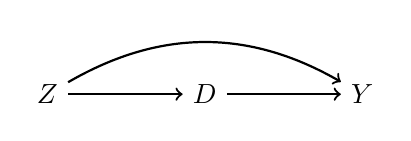
\begin{tikzpicture}[->, node distance=2cm, thick]
        % Nodes
        \node (Z) at (0, 0) {\(Z\)};
        \node (M) at (2, 0) {\(D\)};
        \node (Y) at (4, 0) {\(Y\)};
    
        % Arrows
        \draw[->] (Z) -- (M);
        \draw[->] (M) -- (Y);   
        \draw[->] (Z) to[bend left] (Y);
    \end{tikzpicture}
    \item Direct Effect: $\mathbb{E}[(Y(1, M=m) - Y(0,M=m)]$
    \begin{description}
        \item[Natural effects:] $m = M(1) \text{ or } m = M(0)$
        \item[Controlled effects:] $m \in \mathcal{M}$ (set of all possible values of M)
    \end{description}
    \item Indirect Effect: $\mathbb{E}[(Y(Z, m_1) - Y(Z,m_0)]$
    \begin{description}
        \item[Natural effects:] $m_1 = M(1),~ m_0 = M(0)$
        \item[Controlled effects:] $m_0, m_1 \in \mathcal{M}$
    \end{description}
\end{itemize}

\subsection*{Time-Varying Treatment + Confounding}
ex: HIV patients take antiretroviral medicines on + off over time
ex: candidates adjust their campaign strategy based on polls + opponent's behavior

Suppose we have two time points.\\

\textbf{Temporal order:}
\[
X_0 \to Z_1 \overset{a}{\to} X_1 \to Z_2 \to Y
\]
\begin{itemize}
    \item $X_0$: baseline covariates
    \item $Z_1$: treatment at time point 1 (binary): with 1-4 hours
    \item $X_1$: time-varying covariates observed between treatments
    \item $Z_2$: treatment at time point 2 (binary): with 4-8 hours
    \item $Y$: Outcome
\end{itemize}
4 potential outcomes: Y(0,0), Y(0,1), Y(1,0), Y(1,1)
Observed outcome: 

\textbf{Estimates:}

E[Y($Z_1$, $Z_2$)]
\begin{itemize}
    \item E[Y(1,0) - Y(0,0)]
    \item E[Y(0,1) - Y(0,0)]
    \item E[Y(1,1) - Y(0,0)]
\end{itemize}

Our choice of estimand depends on policy/ science question \\ \\
Suppose our estimate is E[Y($Z_1$, $Z_2$)]

\textbf{Identifications:}
Assumption: Sequential ignorability: treatments are sequentially randomized given observed history 
1. $Z_1$ is randomized given $C(X_0)$.
\[
Z_1 \perp\!\!\!\perp Y(Z_1, Z_0) \mid Z_0, 
\]
for $z_1, z_2 \in \{0, 1\}$.
2. $Z_2$ is randomized given $C(Z_1, X_1, X_0)$.
\[
Z_2 \perp\!\!\!\perp Y(Z_1, Z_0) \mid Z_1, X_1, X_0
\]
for $z_1, z_2 \in \{0, 1\}$

Satisfied under a DAG
\begin{center}
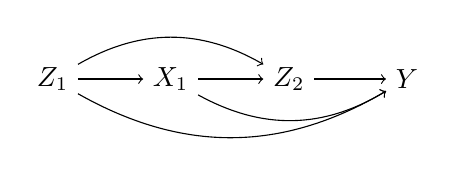
\begin{tikzpicture}[->, node distance=1.5cm]
    % Nodes
    \node (Z1) {$Z_1$};
    \node (X1) [right of=Z1] {$X_1$};
    \node (Z2) [right of=X1] {$Z_2$};
    \node (Y) [right of=Z2] {$Y$};

    % Arrows
    \draw[->] (Z1) -- (X1);
    \draw[->] (X1) -- (Z2);
    \draw[->] (Z2) -- (Y);
    \draw[->, bend right=30] (Z1) to (Y);
    \draw[->, bend right=30] (X1) to (Y);
    \draw[->, bend left=30] (Z1) to (Z2);
\end{tikzpicture}
\end{center}
Also satisfied under OAG
\begin{center}
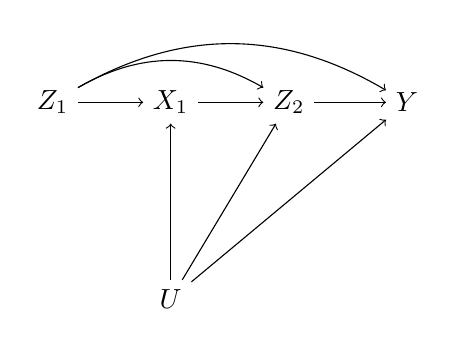
\begin{tikzpicture}[->, node distance=1.5cm]
    % Nodes
    \node (Z1) {$Z_1$};
    \node (X1) [right of=Z1] {$X_1$};
    \node (Z2) [right of=X1] {$Z_2$};
    \node (Y) [right of=Z2] {$Y$};
    \node (U) [below of=X1, yshift=-1cm] {$U$};

    % Arrows
    \draw[->] (Z1) -- (X1);
    \draw[->] (X1) -- (Z2);
    \draw[->] (Z2) -- (Y);
    \draw[->, bend left=30] (Z1) to (Y);
    \draw[->, bend left=30] (Z1) to (Z2);
    \draw[->] (U) -- (X1);
    \draw[->] (U) -- (Z2);
    \draw[->] (U) -- (Y);
\end{tikzpicture}
\end{center}

Recall identification under a single time-point setting:
$\mathbb{E}[Y(Z)] = \mathbb{E}[\mathbb{E}[Y|Z=z,X]]$
\begin{itemize}
    \item discrete X: $\sum_X\mathbb{E}[Y|Z=z,X=x]\mathbb{P}(X=x)$
    \item continuous X: $\int_X\mathbb{E}[Y|Z=z,X=x]p(x)dx$
\end{itemize}
\begin{itemize}
    \item For discrete $X$:
    \[
    \sum_{x} \mathbb{E}[Y \mid Z = z, X = x] P(X = x)
    \]
    \item For continuous $X$:
    \[
    \int_{x} \mathbb{E}[Y \mid Z = z, X = x] p(X) \, dx
    \]
\end{itemize}
\textbf{Theorem}

 Under sequential ignorability:
 $\mathbf{E}[Y(Z_1, Z_2)] = \mathbf{E}\left[\mathbf{E}\left[\mathbf{E}[Y \mid Z_2 = Z_2, Z_1 = Z_1, X_1, X_0] \mid Z_1 = Z_1, X_0\right]\right]$
 
"g-formula" - Jamie Robins:
\begin{itemize}
\item discrete $X_0, X_1$

$=\sum_{X_0}\sum_{X_1}\mathbb{E}[Y|z_2,z_1,X_1,X_0]\mathbb{P}(X_1|z_1,X_0)\mathbb{P}(X_0)$ 
\item continuous $X_0, X_1$

$=\int\int\mathbb{E}[Y|Z_2,Z_1,X_1,X_0]p(X_1|Z_1,X_0)p(X_0)dx_1dx_0$ 
\end{itemize}



\textbf{Proof}
\begin{itemize}
    \item 
\begin{align*}
\mathbb{E}[Y(Z_1,Z_2)] &= \mathbb{E}[\mathbb{E}[Y(Z_1,Z_2) \mid X_0]] \\
&= \mathbb{E}[\mathbb{E}[Y(Z_1,Z_2) \mid Z_1, X_0]] \quad \text{by sequential ignorability} \\
&= \mathbb{E}[\mathbb{E}[\mathbb{E}[Y(Z_1,Z_2) \mid Z_1, X_1, X_0] \mid Z_1, X_0]] \quad \text{by Tower Property} \\
&= \mathbb{E}[\mathbb{E}[\mathbb{E}[Y(Z_1,Z_2) \mid Z_2, Z_1, X_1, X_0] \mid Z_1, X_0]] \quad \text{by sequential ignorability} \\
&= \mathbb{E}[\mathbb{E}[\mathbb{E}[Y \mid Z_2, Z_1, X_1, X_0] \mid Z_1, X_0]]
\end{align*}
\end{itemize}

\subsection*{Estimators}

\subsubsection*{1. Outcome Modeling}

\begin{itemize}
    \item Recall outcome modeling in a single time-point setting:
    \[
    \mathbb{E}[Y(Z)] = \mathbb{E}[\mathbb{E}[Y \mid Z = z, X]]
    \]

    \item Steps:
    \begin{enumerate}
        \item Regress $Y \sim X \mid Z = z$ to obtain $\hat{Y}_i(z)$ for all units.
        \item Compute:
        \[
        \widehat{\mathbb{E}}[Y(Z)] = \frac{1}{n} \sum_{i=1}^n \hat{Y}_i(z)
        \]
    \end{enumerate}
    
    \item Now, in a time-varying setting:
    \begin{enumerate}
        \item Regress $Y \sim X_1, X_0 \mid Z_1 = z_1, Z_2 = z_2$ to get $\hat{Y}_{i2}(z_1, z_2)$.
        \item Regress $\hat{Y}_{i2}(z_1, z_2) \sim X_0 \mid Z_1 = z_1$ to get $\hat{Y}_i(z_1, z_2)$.
        \item Compute:
        \[
        \widehat{\mathbb{E}}[Y(Z_1, Z_2)] = \frac{1}{n} \sum_{i=1}^n \hat{Y}_i(z_1, z_2)
        \]
    \end{enumerate}
\end{itemize}

\subsection*{2. IPW Estimator}

\begin{itemize}
    \item Recall for a single time-point, the identification:
    \[
    \mathbb{E}[Y(Z)] = \mathbb{E}\left[\frac{\mathbb{I}\{Z = z\} Y}{P(Z = z \mid X)}\right]
    \]

    \item For a two-time-point setting:
    \begin{itemize}
        \item Define:
        \[
        e(z_1, X_0) = P(Z_1 = z_1 \mid X_0)
        \]
        \[
        e(z_2, z_1, X_1, X_0) = P(Z_2 = z_2 \mid Z_1 = z_1, X_1, X_0)
        \]
    \end{itemize}

    \item Theorem (under sequential ignorability):
    \[
    \mathbb{E}[Y(Z_1, Z_2)] = \mathbb{E}\left[\frac{\mathbb{I}\{Z_1 = z_1\} \mathbb{I}\{Z_2 = z_2\} Y}{e(z_1, X_0) e(z_2, z_1, X_1, X_0)}\right]
    \]

    \item Highlights the overlap assumption:
    \[
    0 < e(z_1, X_0) < 1, \quad 0 < e(z_2, z_1, X_1, X_0) < 1, \quad \forall z_1, z_2
    \]

    \item IPW Estimator:
    \begin{enumerate}
        \item Regress $Z_1 \sim X_0$ to estimate $\hat{e}(z_1, X_0)$.
        \item Regress $Z_2 \sim Z_1, X_1, X_0$ to estimate $\hat{e}(z_2, z_1, X_1, X_0)$.
        \item Compute:
        \[
        \widehat{\mathbb{E}}[Y(Z_1, Z_2)] = \frac{1}{n} \sum_{i=1}^n \frac{\mathbb{I}\{Z_{1i} = z_1\} \mathbb{I}\{Z_{2i} = z_2\} Y_i}{\hat{e}(z_1, X_{0i}) \hat{e}(z_2, z_1, X_{1i}, X_{0i})}
        \]
    \end{enumerate}
\end{itemize}



\subsection*{Limitations and Solutions}

\subsubsection*{Limitations}
For $K$ time points, we have $2^K$ treatment combinations. This approach may not work well for settings with more than a few time points.

\subsubsection*{Solution: Marginal Structural Model (MSM)}
References:
\begin{itemize}
    \item Robins 2000
    \item Hernán 2000
\end{itemize}

\subsubsection*{Detour:}
Point treatment, continuous, or multivariate/multi-dimensional treatments.

\subsubsection*{Examples:}
\begin{enumerate}
    \item \textbf{Dose:} Drug dose, e.g., mg of aspirin over time.
    \item \textbf{Duration:} e.g., effect of education duration on wages.
    \begin{itemize}
        \item Multidimensional: also degree level (undergrad, master’s, etc.).
    \end{itemize}
    \item \textbf{Frequency:} e.g., estimate effects of hospital nurse staffing on readmission outcomes.
    \begin{itemize}
        \item Nurse staffing = nurse hours/day.
    \end{itemize}
\end{enumerate}
                                    
\Subsection{Identification:}
$\mathbb{E}[Y(Z=z)] = \mathbb{E}[\mathbb{E}[Y|X,Z=z]]$

\Subsection{MSM Estimation:}
\begin{itemize}
    \item Assume a model:
    \[
    \mathbb{E}[Y(Z)] = g(z, \beta)
    \]
    where $g(z, \beta)$ is a known function up to a finite-dimensional parameter $\beta$.
    
    \item Example (Semiparametric model assumption):
    \[
    \mathbb{E}[Y(Z)] = \beta_0 + \beta_1 z + \beta_2 z^2
    \]
\end{itemize}

\subsection*{Semiparametric Approach and IPW Estimator under MSM}

\subsubsection*{Definition}
\[
\beta = \arg\min_\beta \int \left(\mathbb{E}[Y(Z)] - g(Z; \beta)\right)^2 P(Z) dZ
\]

\subsubsection*{Back to the Time-Varying Setting (2 Time Points)}
\paragraph*{Semiparametric Approach}
Assume:
\[
\mathbb{E}[Y(Z_1, Z_2)] = g(Z_1, Z_2; \beta)
\]

\paragraph*{Best Approximation Approach}
\[
\beta = \arg\min_\beta \sum_{z_1} \sum_{z_2} \left(\mathbb{E}[Y(Z_1, Z_2)] - g(Z_1, Z_2, X_0; \beta)\right)^2
\]

\subsubsection*{IPW under MSM with Sequential Ignorability}
\[
\beta = \arg\min_\beta \sum_{z_1} \sum_{z_2} \mathbb{E} \left[\frac{\mathbb{I}\{Z_1 = z_1\} \mathbb{I}\{Z_2 = z_2\}}{e(z_1, X_0) e(z_2, z_1, X_1, X_0)} \left(Y - g(Z_1, Z_2, X_0; \beta)\right)^2 \right]
\]

\subsubsection*{IPW Estimator under MSM}
\begin{enumerate}
    \item Estimate two propensity scores (same as IPW steps described above):
    \begin{itemize}
        \item $e(z_1, X_0) = P(Z_1 = z_1 \mid X_0)$
        \item $e(z_2, z_1, X_1, X_0) = P(Z_2 = z_2 \mid Z_1 = z_1, X_1, X_0)$
    \end{itemize}
    \item $\hat{\beta}$ is the coefficient of a Weighted Least Squares (WLS) fit of:
    \[
    Y_i \sim (1, Z_{1i}, Z_{2i}, X_{0i})
    \]
    with weights:
    \[
    w_i = \frac{1}{\hat{e}(Z_{1i}, X_{0i}) \hat{e}(Z_{2i}, Z_{1i}, X_{1i}, X_{0i})}.
    \]
\end{enumerate}


